\documentclass[authoryear,preprint,review,12pt]{elsarticle}

\usepackage{amssymb}
\usepackage{amsmath}
\usepackage{booktabs}
\usepackage{multirow}
\usepackage{lineno}
\usepackage{hyperref}
\usepackage{graphicx}
\usepackage{tikz}
\usetikzlibrary{arrows.meta, positioning, fit, backgrounds}

\journal{Environmental Modelling \& Software}

\begin{document}

\begin{frontmatter}

\title{nowcast: a forcing-agnostic Rust engine for dynamic geohazard
nowcasting, and what rainfall resolution buys an intensity--duration trigger}

\author[1]{Francisco Parra\corref{cor1}}
\ead{francisco.parra.o@usach.cl}
\cortext[cor1]{Corresponding author}

\affiliation[1]{organization={Departamento de Ingenier\'ia Inform\'atica,
            Universidad de Santiago de Chile},
            city={Santiago},
            country={Chile}}

\begin{abstract}
Landslide and flood susceptibility maps are static: fixed predisposing factors
combined by physical or machine-learning models. Turning susceptibility into an
operational \emph{nowcast} requires modulating it in time with the dynamic
forcing that triggers failure, such as rainfall, snowmelt, routed discharge or
ground deformation. We present \textbf{nowcast}, a dependency-light Rust engine
that writes time-varying hazard as a susceptibility field times a trigger factor,
behind a single interchangeable forcing interface. The hazard logic is thereby
decoupled from the data source and from the trigger family. The engine ships
native providers that wrap sibling Rust models for rainfall--runoff, snowmelt,
2-D shallow-water inundation, an agent-based debris-flow model, a geospatial
raster substrate and PS-InSAR/SBAS deformation. Triggers are composable (rainfall
intensity--duration, discharge, deformation rate), and physical refinement runs
on demand only where the cheap nowcast alerts. We use the engine as an
experimental instrument over Chilean basins, holding the model fixed and varying
the resolution of the forcing. A backtest of 157 dated rainfall-triggered
landslides in the R\'io Maipo basin shows that the global Caine (1980)
intensity--duration threshold fires on only 7 of 13\,880 days, none coinciding with a
recorded event (probability of
detection, POD $=0$), whereas a calibrated regional intercept transfers
split-sample (validation POD $\approx 0.50$) but is not distinguishable from a seasonality-preserving null over the 19 event-months of the record. Distributing that daily forcing
over the basin and weighting by a real machine-learning susceptibility raster
does not improve discrimination. The area under the ROC curve is indistinguishable
from random (AUC $\approx 0.48$; month-block bootstrap 95\,\% CI spans 0.5): at
5\,km daily resolution the gridded rainfall at event cell-months is no higher
than average, and a supervised baseline trained on the same daily features fares
no better (cross-validated AUC $\le 0.56$). Diagnostics show that null accuses the
target as much as the forcing --- recorded events sit at the 46th percentile of
their own cell's history and dilating the label in time and space does not recover
signal --- so we do not rest the resolution claim on it. A controlled experiment whose labels come from an
\emph{independent} failure mechanism, not from the rule under test, isolates why:
aggregating the identical field to daily resolution collapses the catch rate on
burst-driven failures from 0.46 to 0.00 while leaving accumulation-driven failures
untouched at ${\approx}0.42$, with the model and terrain held fixed; the collapse itself follows from the design, since no burst of that size exceeds the curve once spread over a day, so the experiment measures where between half-hourly and daily the catch rate falls and that accumulation-driven failures are spared, not whether daily forcing can ever see a burst. At half-hourly GPM IMERG
resolution the same intensity--duration trigger places the threshold crossing at a
timestamp hours ahead of the documented flows on the same day, a timing that no daily product can give at any
magnitude, because its finest resolvable mean intensity is total$/24$\,h; without an event onset hour and an off-event crossing rate these are timing demonstrations, not skill scores. Across
three dated events spanning opposite Chilean climates we decompose that contrast
one factor at a time, inserting the same satellite series aggregated to 24\,h to
separate the rainfall product from its resolution: resolution governs the timing in
every case and governs detection for a short convective burst, whereas for a
high-magnitude storm it is the product, not the resolution, that decides whether
the curve is crossed at all, and in the first weeks of live operation both half-hourly satellite products missed a convective burst that a rain gauge and the lightning sensor saw. What resolution buys is therefore intra-day timing in general and detection only for short bursts; the magnitude error of the rainfall product, and in operation the sensor, bind elsewhere. The result does not rest on the
threshold chosen either: each event has a measurable band of intercepts, spanning a
factor of 2--3, in which resolution alone decides detection, and the contrast
persists across the published I--D curves of the literature. A complementary flood path,
checked against observed daily streamflow on the R\'io Itata, discriminates
observed floods out of sample (ROC-AUC 0.90) but no better than a 3-day rainfall sum or persistence (0.94--0.95): discharge routing integrates
the rainfall that a sub-daily landslide trigger must instead resolve directly, and the daily forcing is sufficient for it. The
engine, its backtesting framework and the examples behind the core results are open and reproducible from an archived snapshot; the provider crates need the sibling engines.
\end{abstract}

\begin{highlights}
\item A forcing-agnostic Rust engine couples static susceptibility to dynamic triggers
\item Rainfall, snowmelt, discharge and InSAR deformation enter through one interface
\item Distributing daily rainfall does not improve discrimination (AUC $\approx 0.48$)
\item Sub-daily rainfall buys an I--D trigger intra-day timing always, detection only for short bursts
\item Rainfall-product magnitude, not the time step, decides detection in most events
\end{highlights}

\begin{keyword}
nowcasting \sep landslides \sep floods \sep intensity--duration threshold \sep
rainfall resolution \sep Rust \sep early warning \sep Chile
\end{keyword}

\end{frontmatter}

\linenumbers

\section{Introduction}

Operational forecasting of rainfall-triggered geohazards sits between two
well-developed but disjoint bodies of work. On one side, \emph{susceptibility}
mapping combines static predisposing factors (slope, lithology, land cover,
terrain indices) through statistical, physically-based or, increasingly,
machine-learning models, to estimate \emph{where} failures are possible
\citep{reichenbach2018,merghadi2020}. On the other, empirical \emph{rainfall thresholds}, most
famously the intensity--duration (I--D) power law of \citet{caine1980} and its
many regional successors \citep{guzzetti2007,segoni2018,gariano2016}, estimate \emph{when}
triggering rainfall has occurred. Operational early-warning, however, needs
\emph{where} and \emph{when} together, as a hazard field that evolves through an
event; and the \emph{when} itself depends on the hydrological state that prepares a
slope, not only on the meteorological trigger \citep{bogaard2018}. This coupling is already realised operationally: NASA's
LHASA gates a static landslide susceptibility map with GPM IMERG satellite-rainfall
thresholds at the global scale \citep{kirschbaum2018}, its successor adds a
data-driven model \citep{stanley2021}, and geographical landslide early-warning
systems are operational in a growing number of nations and regions \citep{guzzetti2020}. What these share is a
\emph{product-specific} design: the forcing, the trigger and the susceptibility
model are welded into one operational chain, so swapping the rainfall product,
adding a second trigger (snowmelt, discharge, deformation), or attaching a
physical-refinement model means rebuilding the pipeline. The open question is less
\emph{whether} to couple susceptibility and forcing than \emph{how much resolution
the forcing must carry} for the coupling to have skill, a question a fixed
operational chain cannot easily ask.

Closing that gap raises three software problems that recur across hazards and
regions. First, the \emph{forcing} is heterogeneous: a rain gauge, a gridded
reanalysis product, a satellite quantitative precipitation estimate, a
rainfall--runoff hydrograph, or an InSAR deformation field, each with its own
grid, units and time step. Second, the \emph{trigger} family is hazard-dependent:
landslides respond to rainfall I--D, floods to discharge over a threshold, slow
slopes to deformation rate, yet all share the structure ``exceedance of a
critical level mapped to a hazard factor''. Third, validation against dated event
inventories is itself a methods problem with non-obvious metric choices for rare,
spatially sparse, incomplete records.

We present \textbf{nowcast}, a Rust engine that addresses these three problems
with one abstraction (an interchangeable \emph{forcing} interface and a
composable \emph{trigger}), and we then use it as an experimental instrument to
ask a question that the threshold literature has begun to pose with gauge and radar data: holding the model fixed, how much does the
\emph{resolution of the forcing} determine attainable skill? Coarse temporal resolution is known to bias fitted I--D thresholds downward \citep{marra2019,gariano2020}, spatial aggregation and rainfall-estimation uncertainty to shift debris-flow thresholds \citep{marra2017,nikolopoulos2014}, satellite rainfall products to remain some way from operational threshold use \citep{brunetti2018}, and territorial early-warning systems built on such thresholds have been reviewed by \citet{piciullo2018}. Those studies refit the threshold to each dataset; here the trigger is held fixed and the forcing varies one factor at a time, inside an engine that also runs the same trigger online. The contributions
are computational rather than a new hazard law. (1)~A \emph{forcing-agnostic}
design whose random-access forcing trait makes online streaming and dated-event
replay backtesting fall out of one interface, so the same engine is both an
operational nowcaster and an experimental instrument, and the hazard logic never
changes when the rainfall product, the trigger family or the physical-refinement
model is swapped. (2)~A composable multi-trigger with \emph{exact, closed-form}
attribution of every alert, an analytic decomposition into terrain and forcing
drivers that needs no perturbation sampling (contrast SHAP), afforded by the
closed-form hazard. (3)~An on-demand coupling that confines expensive 2-D physics
to the cells the cheap nowcast has already flagged. (4)~A backtesting framework
with metrics appropriate for sparse, month-dated inventories, and the resolution
diagnosis that this instrument makes possible. The established components (the
Caine I--D law, a logistic factor, prefix-sum windows) enter as building blocks
and are not claimed as novel; the contribution is the architecture that makes
them independently swappable and the diagnosis that architecture enables. On real Chilean data, distributing daily forcing and adding real susceptibility does not improve discrimination. That null is diagnosed rather than attributed; a sub-daily head-to-head and a one-factor decomposition then show that resolution governs intra-day timing in every event and detection only for a short burst, with the magnitude error of the rainfall product binding elsewhere. A flood path checked against observed streamflow shows the converse case: where routing integrates the forcing, daily resolution suffices (out-of-sample ROC-AUC 0.90, no better than a 3-day rainfall sum).

\section{The nowcast engine}

\subsection{Hazard formulation}

The engine represents hazard on a row-major raster grid. For every cell and time
step,
\begin{equation}
\mathrm{hazard}(\mathrm{cell},t)=\mathrm{susceptibility}(\mathrm{cell})\times
\mathrm{trigger\_factor}(\mathrm{exceedance},t),
\label{eq:hazard}
\end{equation}
where $\mathrm{susceptibility}\in[0,1]$ is a static background field (a terrain
index, a physically-based factor-of-safety proxy, or a machine-learning
susceptibility raster) and $\mathrm{trigger\_factor}\in[0,1]$ is a dimensionless
modulation derived from the dynamic forcing. Both factors lie in $[0,1]$, so the
product is a bounded hazard index. We call it an \emph{index} because it is not a calibrated probability (Section~\ref{sec:limits}).

The trigger factor is a smooth function of an \emph{exceedance ratio} $E$, how
far the forcing has crossed a critical level. A hard threshold ($E\geq 1$ fires,
else nothing) discards how far past the curve the forcing reached; instead we use
a logistic,
\begin{equation}
\mathrm{trigger\_factor}(E)=\frac{1}{1+\exp\!\big(-k\,(E-1)\big)},
\label{eq:logistic}
\end{equation}
with $\mathrm{trigger\_factor}(1)=0.5$ exactly on the curve and steepness $k$
(default 4). The \emph{source} of $E$ is what varies between hazards.

\subsection{The forcing interface}

A single trait abstracts the dynamic forcing as a per-cell, per-step scalar field
with a known time step:
\begin{verbatim}
pub trait Forcing {
    fn dims(&self) -> GridDims;
    fn n_steps(&self) -> usize;
    fn dt_hours(&self) -> f64;
    fn depth_mm(&self, cell: usize, step: usize) -> f64;
}
\end{verbatim}
The trait offers random access, not a pull or iterator model, because the I--D logic accumulates rolling windows and backtesting replays whole dated series. Shipped
implementations are a single observed gauge broadcast over a grid, an independent
series per cell (a gridded precipitation product) and, through the provider
crates, snowmelt runoff and InSAR deformation. The same trait therefore admits a
gauge, a reanalysis grid, a satellite product or a model output without touching
the hazard logic (Fig.~\ref{fig:arch}).

\paragraph{Relation to model-coupling standards}
Standardised interfaces for coupling environmental models are long established:
OpenMI \citep{gregersen2007} defines a link-based standard for exchanging
time-varying quantities between running components, the CSDMS Basic Model
Interface \citep{peckham2013,hutton2020} prescribes a small set of
initialise/update/get--set functions that any model implements to become
composable, and the Object Modeling System \citep{david2013} approaches the same
problem from a software-engineering direction, using lightweight annotations
instead of a prescriptive component API. We do not propose \texttt{Forcing} as an
alternative to these. It is narrower: a read-only, random-access view of \emph{one} scalar field, with no lifecycle, no time control and no bidirectional exchange. That narrowness is what makes random access cheap, and both the I--D window kernel and the backtester depend on it. The trade is the usual one. A single-purpose interface is trivial for a provider to implement (each of our adapters is a few dozen lines), but it cannot express two-way coupling or let a component drive the clock, and those are the jobs BMI and OpenMI exist to do. The two levels compose rather than compete: a BMI-exposed model is a
legitimate source behind a \texttt{Forcing} implementation, and wrapping the
engine itself in BMI so that it can be driven inside a CSDMS or OpenMI
composition is the natural interoperability step, left as future work.

\begin{figure}[t]
\centering
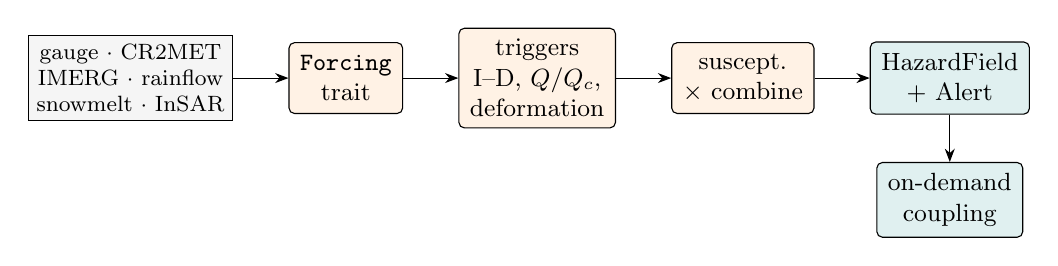
\begin{tikzpicture}[font=\small, >=Stealth,
  box/.style={draw, rounded corners=2pt, align=center, inner sep=4pt, minimum height=9mm},
  src/.style={draw, align=center, inner sep=3pt, font=\footnotesize, fill=black!4},
  core/.style={box, fill=orange!10},
  outbox/.style={box, fill=teal!12}]
\node[src] (forc) {gauge $\cdot$ CR2MET\\ IMERG $\cdot$ rainflow\\ snowmelt $\cdot$ InSAR};
\node[core, right=7mm of forc] (trait) {\texttt{Forcing}\\ trait};
\node[core, right=7mm of trait] (trig) {triggers\\ I--D, $Q/Q_c$,\\ deformation};
\node[core, right=7mm of trig] (haz) {suscept.\\ $\times$ combine};
\node[outbox, right=7mm of haz] (alert) {HazardField\\ + Alert};
\node[outbox, below=6mm of alert] (couple) {on-demand\\ coupling};
\draw[->] (forc)--(trait); \draw[->] (trait)--(trig); \draw[->] (trig)--(haz);
\draw[->] (haz)--(alert); \draw[->] (alert)--(couple);
\end{tikzpicture}
\caption{Engine dataflow. Heterogeneous forcings enter through one
\texttt{Forcing} interface; composable triggers map each to an exceedance factor;
their combination modulates the static susceptibility into a per-step
\texttt{HazardField} and \texttt{Alert}s. Where an alert fires, a process model is
run on demand to refine it (2-D shallow water for floods, an agent-based
debris-flow model for landslides). The geospatial substrate (GeoTIFF I/O, CRS)
moves rasters in and out.}
\label{fig:arch}
\end{figure}

\subsection{The rainfall intensity--duration trigger}

For rainfall-triggered landslides the exceedance is computed against a power-law
I--D curve,
\begin{equation}
I_{\mathrm{crit}}(D)=a\,D^{-b}\qquad(I\;\mathrm{in\;mm\,h^{-1}},\;D\;\mathrm{in\;h}),
\label{eq:id}
\end{equation}
with the \citet{caine1980} global intercept $a=14.82$, $b=0.39$ as a default,
replaceable by a regional curve. For each cell and step, the engine accumulates
water input over rolling windows of length $m=1\ldots m_{\max}$ ending at that
step, forms the mean intensity $I=\mathrm{depth}/(m\,dt)$ and duration $D=m\,dt$,
evaluates $E_m=I/I_{\mathrm{crit}}(D)$, and takes the worst (maximum) exceedance
over all windows; per-cell prefix sums make each window sum $O(1)$.

\subsection{Composable triggers}

The engine generalises the trigger to \emph{composable exceedance sources}. A
\texttt{Trigger} yields a factor per cell and step; an \texttt{IdTrigger}
implements the rolling-window I--D logic above; a \texttt{ThresholdTrigger}
implements a duration-independent exceedance $E=\mathrm{value}/\mathrm{value_{crit}}$
suitable for any signal already expressed as a rate (routed discharge $Q/Q_c$,
InSAR velocity $|v|/v_{\mathrm{crit}}$). A \texttt{MultiNowcast} fuses several
triggers through a combination rule before modulating susceptibility:
\begin{equation}
\mathrm{hazard}=\mathrm{susceptibility}\times\mathrm{combine}(f_1,\ldots,f_k),
\quad\mathrm{combine}\in\{\max,\ \mathrm{noisy\text{-}OR},\ \mathrm{product}\}.
\label{eq:multi}
\end{equation}
Noisy-OR ($1-\prod(1-f_i)$) is the natural rule for independent triggers where
any one may fire, for example \emph{rain I--D} OR \emph{deformation rate}. The
per-trigger factors are exposed for traceability.

\subsection{Physical refinement on demand}

The susceptibility$\times$trigger product is a fast, coarse screen. Where it
alerts, the engine couples, one-way and on demand, to a process model that
refines the alert into a physical field, only over the alerted area. For
\textbf{floods}, a 2-D shallow-water solver (HLLC fluxes, Audusse well-balanced
reconstruction \citep{audusse2004}, semi-implicit Manning friction) routes the
alerting discharge over the local digital elevation model and returns an inundation depth per cell. The solver, hydroflux, and its verification against analytical and community benchmarks are described in a separate manuscript currently under review in this journal; here it is used only as a coupled component. For \textbf{landslides/debris flows}, an agent-based
model (rain and flow agents over the terrain raster, calibrated on the 2015
Atacama event) returns the runout footprint. That calibration feeds only the
runout-footprint demonstration and is independent of the I--D lead-time analysis
(Section~5.4), which uses the rainfall trigger alone. In both, the coarse probability is
downscaled onto the physical footprint; the expensive model runs only where the
cheap nowcast already alerted. The saving is the point and is quantifiable:
because the shallow-water solver integrates to a fixed physical time with
CFL-limited steps, its cost is ${\sim}O(\mathrm{cells})$, so confining it to an
alerted tile spanning 31\,\% of a coarse domain runs $3.8\times$ faster than
solving the full domain (1.19\,s to 0.31\,s; a strictly linear cost would predict $3.2\times$) while returning \emph{bit-identical}
depths in the inundated region, the flood being contained within the tile. The
on-demand restriction is therefore free in accuracy, and the cheap
susceptibility$\times$trigger screen is what keeps the alerted area, and hence the
hydrodynamic cost, small.

\subsection{Exact attribution}

Because Eq.~\eqref{eq:hazard} is closed-form, every alert is \emph{exactly}
attributable, there is no surrogate model to approximate, as post-hoc methods
such as SHAP \citep{lundberg2017} require for black boxes. For any cell and step
the engine reports the two factors, the rolling I--D window that drove the trigger
(its duration, mean intensity, critical intensity and exceedance), which
side, terrain or forcing, is the binding constraint, and a counterfactual: the
rainfall intensity, at a given duration, that would lift the cell to the alert
level. SHAP remains relevant one layer upstream, explaining the machine-learning
\emph{susceptibility} that enters Eq.~\eqref{eq:hazard} as an
already-interpretable input.

\subsection{Implementation}

The engine is written in Rust (edition 2024) as a Cargo workspace of twelve
crates. The core depends only on \texttt{std} and an error-handling crate, so it builds and tests offline with no system dependencies. Native providers are separate crates that wrap sibling engines through path dependencies:
rainfall--runoff (GR4J/HBV; \citealp{perrin2003,seibert2012}), distributed
snowmelt, 2-D shallow water \citep{audusse2004,toro1994}, an agent-based
debris-flow model in the cellular-automata tradition \citep{dambrosio2003}, the SurtGIS geospatial raster substrate \citep{parra2026surtgis} (native GeoTIFF I/O, no GDAL dependency), PS-InSAR/SBAS deformation \citep{ferretti2001,berardino2002}, and a wildfire-spread model (Rothermel surface-fire spread \citep{andrews2018} with a minimum-travel-time perimeter algorithm \citep{finney1998}) with a post-fire susceptibility cascade. A command-line runner exposes the engine (run, backtest, explain, watch, calibrate), and PyO3 bindings expose it to Python. The codebase is covered by $\sim$150 unit, integration and documentation tests, the linter runs clean under \texttt{-D warnings}, and thirty-six runnable examples reproduce every result below.
Each provider is a dependency-isolated crate implementing the same \texttt{Forcing}
trait, so the design is reusable and extensible by construction: adding a hazard
forcing is a new crate, not an edit to the core. That separation, not any single
algorithm it orchestrates, is the engine's computational contribution.

\subsection{Computational performance}

The I--D engine is $O(\mathrm{cells}\times\mathrm{steps}\times m_{\max})$: per-cell
prefix sums reduce each rolling-window sum to $O(1)$, and memory is
$O(\mathrm{cells}\times\mathrm{steps})$ for the prefix buffer. On a single core
(release build, $m_{\max}=7$), throughput is roughly constant at
${\sim}3.7$~million cell-steps per second, confirming the linear scaling
(Table~\ref{tab:perf}). In practice the lumped Maipo backtest (270 cells $\times$
13\,880 daily steps $\approx 3.7$~M cell-steps) runs in about one second, and a
seasonal continental-scale run (490\,k cells $\times$ 365 steps $\approx$
179~M cell-steps) in under a minute. An optional Rayon backend
(\texttt{--features parallel}) parallelises the independent per-step loop; the
closure captures only the read-only prefix buffer, so the output is bit-identical
to the serial run. The speed-up is, however, modest and bandwidth-bound: on a
16-core machine over a 50~M cell-step grid it reaches $1.8\times$ on 2 threads
(88\,\% efficiency) but saturates at $2.8\times$ on 16 threads
(Table~\ref{tab:scaling}), because each step does little arithmetic per byte read
and the shared prefix buffer makes the loop memory-bandwidth-bound rather than
compute-bound. The $O(\mathrm{cells}\times\mathrm{steps})$ prefix buffer
(${\sim}1.4$~GB at the largest size above) is the practical memory limit,
mitigated by chunking the time axis; that same memory pressure, not a lack of
parallel work, is what caps the multi-thread speed-up.

\begin{table}[ht]
\centering
\caption{Single-thread runtime of \texttt{Nowcast::run} over synthetic grids.}
\label{tab:perf}
\begin{tabular}{@{}rrrrr@{}}
\toprule
cells & steps & cell-steps & time (s) & M\,cell-steps\,s$^{-1}$ \\
\midrule
10\,000  & 60  & 0.6\,M   & 0.17  & 3.5 \\
90\,000  & 200 & 18\,M    & 4.7   & 3.8 \\
250\,000 & 200 & 50\,M    & 11.2  & 4.5 \\
490\,000 & 365 & 179\,M   & 48.1  & 3.7 \\
\bottomrule
\end{tabular}
\end{table}

\begin{table}[ht]
\centering
\caption{Parallel scaling of \texttt{Nowcast::run} (\texttt{--features parallel})
over a 50~M cell-step grid, 16-core machine, best of two runs (a separate run from
Table~\ref{tab:perf}: the single-thread time differs by run-to-run variation, 10.5 against 11.2\,s). Output is verified
bit-identical to the single-thread run.}
\label{tab:scaling}
\begin{tabular}{@{}rrrr@{}}
\toprule
threads & time (s) & speed-up & efficiency \\
\midrule
1  & 10.5 & 1.0$\times$ & 100\,\% \\
2  & 6.0  & 1.8$\times$ & 88\,\% \\
4  & 5.2  & 2.0$\times$ & 50\,\% \\
8  & 4.2  & 2.5$\times$ & 31\,\% \\
16 & 3.7  & 2.8$\times$ & 18\,\% \\
\bottomrule
\end{tabular}
\end{table}

\section{Data and study area}

All experiments use openly documented Chilean datasets (Table~\ref{tab:data}).
Susceptibility is a RandomForest probability raster at 30\,m resolution (values
0.001--0.965 over the R\'io Maipo basin, $5149\times5855$ cells), taken from a
companion susceptibility study: the model is trained on landslide presence points
from the SERNAGEOMIN catalogue (augmented with the Patagonian-Andes and 2010 Maule
co-seismic inventories) against spatially-interspersed absence points and terrain,
geology and climate predictors, under spatial cross-validation. This raster is
therefore \emph{not independent} of the validation inventory: it was trained on a
superset of the same dated events the backtest scores against. The dependence is,
however, \emph{conservative} for our purpose. Leakage can only \emph{inflate} the
susceptibility's apparent agreement with event locations, so an inventory-informed
susceptibility that still fails to discriminate at 5\,km daily resolution
(Section~5.2) strengthens the resolution-ceiling conclusion rather than weakening
it; we flag the single place the dependence could matter (the weak single-feature
susceptibility signal in the baseline) where it arises. Daily
precipitation is CR2MET v2.5 (0.05$^\circ$, $\sim$5\,km; \citealp{boisier2018cr2met}), produced over a basin
region that has experienced a sustained decline in rainfall since 2010, the
Central Chile Mega Drought \citep{garreaud2019,boisier2018}.
Sub-daily precipitation is GPM IMERG Final v07 half-hourly ($\sim$0.1$^\circ$;
\citealp{huffman2023,tan2019}). Catchment forcing for the flood path uses CAMELS-CL
\citep{alvarez2018}. The dated event inventory is the SERNAGEOMIN
landslide/flow catalogue, consistent with regional patterns of rainfall-triggered
fatal landslides across Chile and Latin America \citep{sepulveda2015}; events are dated to year and month from the record
identifier, and the month itself is only approximate: the Atacama event flows,
for instance, are filed under March even though the extreme rainfall fell over
24--26 March 2015.

\begin{table}[ht]
\centering
\caption{Datasets.}
\label{tab:data}
\begin{tabular}{@{}llll@{}}
\toprule
Dataset & Variable & Resolution & Use \\
\midrule
RandomForest susceptibility & susceptibility & 30\,m & static background \\
CR2MET v2.5 & daily precipitation & 0.05$^\circ$, daily & lumped \& distributed forcing \\
GPM IMERG Final v07 & precipitation rate & $\sim$0.1$^\circ$, 30\,min & sub-daily forcing \\
CAMELS-CL & precip, PET, streamflow & catchment, daily & flood path (GR4J/HBV) \\
SERNAGEOMIN inventory & dated events & point, $\sim$month & validation target \\
\bottomrule
\end{tabular}
\end{table}

Study sites are the R\'io Maipo basin (central Andes, landslide backtest), the
R\'io Itata catchment (humid south-central, flood path), and three dated
debris-flow events spanning opposite climates: Atacama/Copiap\'o (25 March 2015,
arid, convective), Caj\'on del Maipo (25 February 2017, central Andes, summer
convective) and Villa Santa Luc\'ia (16 December 2017, humid south, frontal). They
span roughly $27^\circ$S to $43^\circ$S, from the hyper-arid Atacama to the humid
Patagonian Andes (Fig.~\ref{fig:studyarea}).

\begin{figure}[t]
\centering
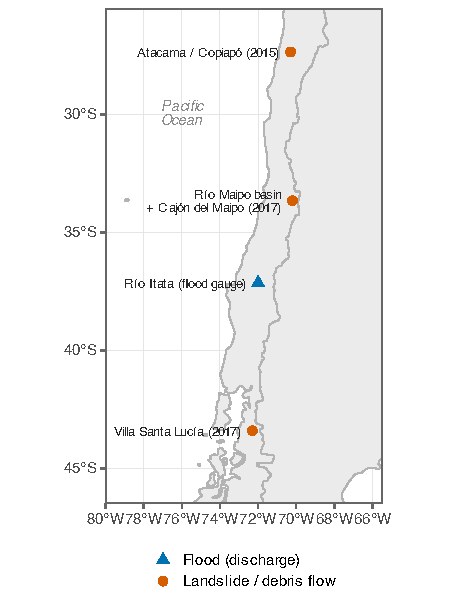
\includegraphics[width=0.48\linewidth]{figs/fig1_studyarea.pdf}
\caption{Study sites in Chile, spanning the arid north to the humid south. Orange:
landslide/debris-flow sites, the R\'io Maipo landslide backtest, which also hosts the
25 February 2017 Caj\'on del Maipo event, the 25 March 2015 Atacama/Copiap\'o event
and the 16 December 2017 Villa Santa Luc\'ia event. Blue: the R\'io Itata
flood-validation catchment (CAMELS-CL gauge 8123001).}
\label{fig:studyarea}
\end{figure}

\section{Methods}

\subsection{Backtesting metrics}

Validation of a nowcast is binary forecast verification, giving a $2\times2$
contingency table and the standard categorical scores, probability of detection
(POD), false-alarm ratio (FAR), critical success index (CSI), frequency bias.
Because the inventory is dated only to $\sim$month, the matching unit is the
calendar month, and matching is \emph{event-centred} with a $\pm$tolerance window
(an event is a hit if an alert falls within the window; a false alarm is an
alerted month far from any event) to avoid inflating misses when one event spans
a tolerance window. For \emph{spatial} verification, per-cell month matching
against a spatially sparse, \emph{incomplete} inventory makes CSI/FAR
meaningless, almost every ``false alarm'' is a susceptible, wet cell with no
\emph{recorded} event. We therefore score discrimination, as the susceptibility
and early-warning literatures do \citep{reichenbach2018}: ROC-AUC \citep{hanley1982} (does the hazard
rank event cell-months above quiet ones?) and POD at a fixed alerted-area
fraction. Uncertainty on the AUC is estimated by a \emph{month-block} bootstrap
(resampling calendar months with replacement, keeping each month's cells
together) so that within-month spatial autocorrelation, the dominant structure
when one storm wets many cells, is not mistaken for independent information. As a
model-agnostic check, we also train supervised baselines (logistic regression and
gradient boosting \citep{friedman2001}) on per-cell-month susceptibility and rainfall features,
evaluated by year-blocked \texttt{GroupKFold} cross-validation, chosen over a
plain random split to avoid leaking within-year spatial autocorrelation across
folds \citep{roberts2016}.

We distinguish two notions used throughout the results. \emph{Triggering} asks
whether the forcing can cross the I--D curve at all; it is a property of the
intensity at the finest resolvable duration, and a daily product can fail it
structurally (Section~5.4). \emph{Discrimination} (or skill) asks the harder
question of whether the resulting hazard \emph{ranks} event locations above
non-event ones, as ROC-AUC and POD measure. The two are not interchangeable: a
forcing can trigger frequently yet discriminate poorly. The distributed backtest
(Section~5.2) tests discrimination on real but month-dated data; a controlled
synthetic experiment (Section~5.3) tests it under known ground truth; the
head-to-head (Section~5.4) isolates triggering.

\subsection{Threshold calibration and split-sample validation}

The I--D intercept $a$ is calibrated by sweeping it (fixed $b=0.39$) and selecting
the value that maximises CSI against the dated events; $k=4$ and a maximum rolling
window of 7\,days (storm I--D durations, not seasonal accumulation) are fixed.
The steepness $k$ enters only through the trigger factor (Eq.~\ref{eq:logistic}),
which is monotonic in the exceedance, so the rank-based discrimination scores
(ROC-AUC, POD at a fixed area) are \emph{exactly} invariant to $k$ for the
trigger-only configuration, where the hazard is a monotone function of exceedance;
$k$ enters the threshold-based POD/FAR only through the chosen alert level.
Validation is split-sample: the intercept is calibrated on odd calendar years and
evaluated on even years.

\section{Results}

\subsection{Lumped landslide backtest (R\'io Maipo)}
\label{sec:lumped}

Over 13\,880 daily steps (1979--2016) and 157 dated rainfall-triggered events, the
global Caine threshold ($a=14.82$) is crossed on only \textbf{7 of 13\,880 days} on CR2MET daily forcing
(POD $=0$): at 24\,h duration the curve sits at $I_{\mathrm{crit}}=4.29$\,mm\,h$^{-1}$, a daily
total of 103\,mm, which only those seven days reach, and none of them falls in an
event month. A regional intercept $a^\star\approx5.5$\,mm\,h$^{-1}$
maximises CSI on the full period and on the odd years alike, and the even-year
validation gives POD $\approx 0.50$ (Fig.~\ref{fig:idsweep}); but the objective is
flat (CSI 0.06--0.08 over $a=2$--13\,mm\,h$^{-1}$), so $a^\star$ is weakly
identified, and the scores carry wide intervals over the 19 event-months of the
record: at $\pm1$ month, POD 0.53 [0.32, 0.73] and FAR 0.92 [0.85, 0.95]
(Wilson 95\,\%). The false-alarm ratio is structural: with an event base rate near 4\,\% of months and a
single representative gauge in a Mediterranean wet-season climate, an I--D trigger
alone over-predicts (126 alert-months, 28\,\% of the record). Whether it
discriminates beyond seasonality is the harder question, and the answer is marginal.
Against a year-shuffle null that keeps the seasonality and the within-year
clustering of the alert-months but reassigns them to random years (2\,000
permutations), the observed CSI of 0.077 is exceeded in 10.5\,\% of permutations
(null POD mean 0.46, 95th percentile 0.58), and an alerter that fires on every
May--September month reaches POD 0.47 at the same tolerance. The inventory's
month-level dating still caps what any trigger can score here, but the rise of
POD with the match tolerance ($0.21\to0.68$ from $\pm0$ to $\pm3$ months,
Table~\ref{tab:lumped}) is not evidence of it: the null rises the same way
($0.27\to0.68$), as does an independent alerter at the same monthly rate
($0.28\to0.90$). The lumped backtest therefore shows that $a^\star$ fires the
trigger in the right season, not that it separates event months from the rest of
the wet season; that is the discrimination question the distributed backtest and
the controlled experiment take up.

\begin{table}[ht]
\centering
\caption{Lumped Maipo backtest (monthly contingency, $\pm1$-month match unless noted).}
\label{tab:lumped}
\begin{tabular}{@{}lccl@{}}
\toprule
Configuration & POD & FAR & note \\
\midrule
Caine global, $a=14.82$ & 0.00 & 1.00 & fires 7/13\,880 d, none on event month \\
Regional $a^\star=5.5$ (full period) & 0.53 [0.32, 0.73] & 0.92 [0.85, 0.95] & max-CSI calibration; 19 event-months, Wilson 95\,\% \\
Regional $a^\star=5.5$ (split-sample) & 0.50 & 0.93 & calibrate odd $\to$ validate even \\
$a^\star=5.5$, tol. $\pm0/\pm1/\pm2/\pm3$\,mo & \multicolumn{2}{c}{POD 0.21/0.53/0.58/0.68} & rises like the nulls below \\
Year-shuffle null, $\pm0/\pm1/\pm2/\pm3$\,mo & \multicolumn{2}{c}{POD 0.27/0.46/0.56/0.68 (mean)} & 2\,000 perm.; $P(\mathrm{CSI}\geq0.077)=0.105$ at $\pm1$ \\
Wet-season alerter (May--Sep), $\pm1$\,mo & 0.47 & 0.95 & 190 alert-months, no rainfall \\
\bottomrule
\end{tabular}
\end{table}

\begin{figure}[t]
\centering
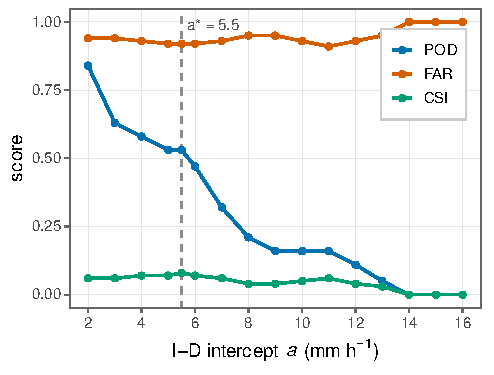
\includegraphics[width=0.62\linewidth]{figs/fig2_idsweep.pdf}
\caption{Calibration of the I--D intercept $a$ on the lumped Maipo backtest
(monthly contingency, $\pm1$-month match). POD falls and false-alarm ratio stays
high across the sweep; the critical success index is flat (0.06--0.08 over $a=2$--13\,mm\,h$^{-1}$) with its maximum at $a^\star\approx5.5$\,mm\,h$^{-1}$
(dashed line), far below the Caine global value of 14.82: the intercept is weakly identified by this objective (Section~\ref{sec:lumped}).}
\label{fig:idsweep}
\end{figure}

\paragraph{Published thresholds do not rescue daily forcing}
Self-calibration invites the objection that a published threshold, taken as is,
might do better. We tested this directly by applying, unchanged, the 35 empirical
I--D power laws ($I=a\,D^{-b}$, mm\,h$^{-1}$) compiled by \citet{guzzetti2007}
(the pure power laws of their Table~2, excluding its asymptotic and normalised
forms) to the same CR2MET
daily forcing. The outcome is dictated by resolution, not by the curve: 10 of the
35 sit \emph{structurally} above the daily ceiling --- on a basin whose wettest
day in 38 years is 136\,mm, no daily forcing can reach their 24\,h intensity, since
the maximum resolvable 24\,h intensity is the daily total divided by 24 --- and 5
never fire at all. Thirteen yield POD $=0$, and of the curves that do fire, 30 have
FAR $\geq 0.90$. The best-scoring published curve attains CSI $=0.084$,
indistinguishable from the self-calibrated regional intercept (CSI $=0.077$): the
entire ensemble is pinned near the same low operating point. A curve high enough to
be selective sits above the wettest day (POD $0$); lowered enough to fire, it fires
on most wet months (FAR $\to 1$). The binding constraint is the forcing resolution,
not the choice of published threshold (\texttt{published\_thresholds} example). The
same 35 curves are re-used in Section~\ref{sec:intercept} to show that the sub-daily
results do not hinge on the choice of curve either.

\subsection{Distributed daily backtest: a null result}

Repeating the backtest with \emph{distributed} CR2MET rainfall over a
$15\times18$ grid (270 cells, 123\,120 cell-months, 884 in the event footprint),
the \emph{real} RandomForest susceptibility resampled to that grid, and spatial
verification, yields essentially \textbf{no discrimination}
(Table~\ref{tab:auc}): ROC-AUC is 0.463 for a lumped basin-mean baseline
weighted by susceptibility, 0.477 for distributed rainfall with uniform
susceptibility, and 0.485 for distributed rainfall weighted by real
susceptibility. A month-block bootstrap (resampling months with replacement, so
within-month spatial autocorrelation is preserved; $B=2000$) puts all three 95\,\%
confidence intervals across the random 0.5 ($[0.40, 0.57]$ for the best
configuration), and the bootstrap probability that AUC exceeds 0.5 is only
0.21--0.34. None of the configurations is distinguishable from random. The mean
7-day rainfall at recorded event cell-months (39\,mm) is in fact \emph{lower}
than the grid-wide average (49\,mm).

\paragraph{What this null does, and does not, accuse}
That last number needs scrutiny. If recorded events sit where it rained \emph{less}, the finger points at the inventory or the rainfall field, not at the time step, and reading it as evidence for a resolution argument would be self-serving. We therefore tested the competing explanations
on the same data (\texttt{null\_diagnosis} example). \emph{Is it a dry cell or a dry
month?} Removing the spatial gradient by standardising each cell against its own
history leaves the null intact (AUC 0.472; the mean event-month anomaly is
$z=-0.13$), so there is no temporal signal being masked by the space dimension.
\emph{Is the record merely displaced?} Dilating the \emph{label} --- counting a
cell-month as positive if an event is recorded within $\pm k$ months and $r$ cells
--- lifts AUC only to 0.496 at $\pm2$ months and one cell of slack, still
indistinguishable from chance, so the events are not just mis-filed by a month or a cell. \emph{Is it exposure bias?} Cells that ever record an event receive
essentially the same climatological rainfall as the rest ($-0.2$\,\%), though they
are slightly more susceptible (0.351 vs 0.329), so the inventory is not
concentrated in a systematically drier part of the basin. Most directly, a recorded
event cell-month sits at the 46th percentile of its own cell's history and the 45th
percentile of its own month's spatial distribution: on both axes it is where chance
would put it.

The conclusion that follows is stronger and narrower than the one this null is often asked to support. The daily 5\,km field carries no recoverable information about
where and when these events were recorded, and no reasonable relaxation of the
label recovers any; but that is a statement about \emph{this target and this
product jointly}, and it cannot be attributed to temporal resolution alone. The
evidence for the resolution claim comes instead from the controlled experiment,
where the labels are generated by a known process (Section~\ref{sec:synthetic}),
and from the single-factor field decomposition
(Section~\ref{sec:singlefactor}). We report the distributed null because a method
paper should show where its instrument reads nothing, not because it proves the
thesis.

\begin{table}[ht]
\centering
\caption{Distributed-backtest discrimination (ROC-AUC) with month-block
bootstrap 95\,\% confidence intervals ($B=2000$). Every interval spans 0.5.}
\label{tab:auc}
\begin{tabular}{@{}lccc@{}}
\toprule
configuration & AUC & 95\,\% CI & $P(\mathrm{AUC}>0.5)$ \\
\midrule
lumped (basin-mean) $\times$ susc. & 0.463 & $[0.375, 0.550]$ & 0.21 \\
distributed, susc.\ $=1$           & 0.477 & $[0.399, 0.560]$ & 0.30 \\
distributed $\times$ real susc.    & 0.485 & $[0.403, 0.565]$ & 0.34 \\
\bottomrule
\end{tabular}
\end{table}

A supervised baseline confirms this is a property of the data, not of our
trigger. Logistic regression and gradient boosting trained on per-cell-month
features (susceptibility; monthly total; maximum 1-day and 7-day rainfall;
previous-month total), evaluated with year-blocked \texttt{GroupKFold}, reach a
cross-validated AUC of only 0.56 and 0.52, barely above random. A single-feature
analysis locates the little signal that exists: it comes from the static
susceptibility (AUC 0.55, itself an optimistic upper bound since this raster was
trained on the same inventory, Section~3) and weak antecedent wetness (0.52),
whereas every rainfall-intensity feature is at or below random (max 7-day 0.49,
max 1-day 0.46, monthly total 0.46). The daily rainfall therefore carries essentially no
information about where and when these landslides occurred, and a flexible model
cannot recover a signal the daily product does not contain. Our engine's 0.485
even dips slightly below susceptibility alone, because multiplying susceptibility
by a near-random daily-rainfall factor dilutes it: at this resolution the daily
trigger is worse than none.

\begin{figure}[t]
\centering
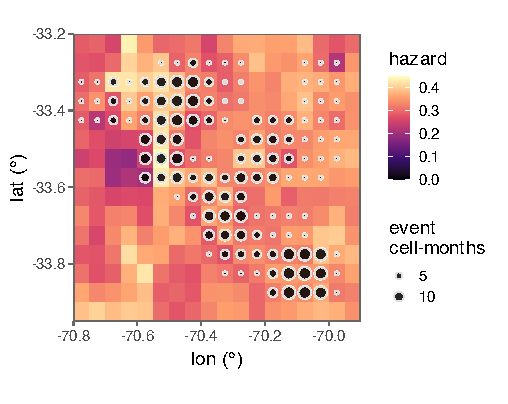
\includegraphics[width=0.6\linewidth]{figs/fig4_hazard.pdf}
\caption{Example distributed hazard field over the R\'io Maipo event region
(15$\times$18 CR2MET grid) at the wettest step, with real RandomForest
susceptibility and the regional I--D trigger ($a=5.5$); dots mark the cells of
the inventory footprint, sized by their number of recorded event cell-months
(884 over 129 cells). No cell reaches the 0.5 alert level at this step. The field is
spatially structured, yet at 5\,km daily resolution it does not separate the
recorded event cell-months (Section~5.2); Fig.~\ref{fig:synthetic} shows, on
controlled data, how that discrimination returns as resolution increases.}
\label{fig:hazard}
\end{figure}

\subsection{Controlled resolution experiment}
\label{sec:synthetic}

The distributed null is ambiguous on its own: a near-random AUC could mean the
engine has no skill, or that the month-dated, incomplete inventory cannot reveal
skill that is present. We resolve the ambiguity with a controlled experiment whose
ground truth is known.

\paragraph{The labels do not come from the rule under test}
A synthetic experiment that defines an event as ``a burst that crosses the I--D
curve'' and then reports that an I--D trigger recovers it is deductive: the result
is entailed by the construction, not evidence about it. We therefore generate the
labels with an \emph{independent} failure mechanism. On a $20\times20$ grid over 60
days we synthesise one half-hourly rainfall field with two day types --- a
${\sim}1$\,h burst (8--30\,mm) and a similar-to-larger total (16--46\,mm) smeared
over 8--23\,h --- and then decide failure with a transient pore-pressure analogue:
a linear store fed by capped infiltration (excess runs off) and drained with a
${\sim}4$\,h time constant, failing the cell-day when it exceeds
$\theta_\mathrm{crit}=12$\,mm. This is a different functional form from
$I=a\,D^{-b}$, and the two do not coincide: per realisation about 123 of 667 bursts
never fail, and about 1167 failures fall on days that were \emph{not} bursts, so the
label is not a relabelling of the day type. Critically, the store is always
integrated at the native half-hourly step --- the physics happens at full
resolution and it is the \emph{observation} we degrade. Susceptibility is
structured but uncorrelated with which days fail, so it carries no separating
information. We then aggregate the identical field from 0.5\,h to 24\,h, holding
the engine and the 24\,h maximum duration fixed, and score against the physical
labels over 20 random realisations (Fig.~\ref{fig:synthetic}).

\paragraph{Aggregation destroys one failure route and spares the other}
The store fails cell-days by two paths: a burst outrunning drainage, and slower
rain accumulating past $\theta_\mathrm{crit}$. Aggregation does not treat them
alike, and that is the result. \textbf{Stratified by mechanism, the operational
catch rate on burst-driven failures collapses from $0.46\pm0.09$ at half-hourly to
$0.00\pm0.01$ at daily, while accumulation-driven failures are caught at
${\approx}0.42$ at \emph{every} resolution} (POD at a 5\,\% alerted-area budget).
The collapse itself is expected from the design and we do not present it as a discovery: no burst in the 8--30\,mm range exceeds the $a^\star$ curve once spread over 24\,h (the largest gives $E=0.79$; crossing the daily ceiling at $a^\star=5.5$ takes 38\,mm in a day), so what the experiment measures is where between half-hourly and daily the catch rate falls, and that accumulation-driven failures are spared, not whether daily forcing can ever see a burst. Bursts large enough to cross the daily ceiling are the 7 Maipo days of Section~\ref{sec:lumped}. Moving the design knobs one at a time (Table~\ref{tab:sweep}; five realisations each) says where the collapse lives. It is a property of the burst magnitude relative to the daily ceiling: with bursts of 30--60\,mm, straddling the ceiling, the daily catch rate on burst-driven failures stays at 0.46, and with bursts of 60--120\,mm the daily product scores \emph{higher} than the half-hourly one (0.70 against 0.47), because a burst that dominates its day is easier to rank at the coarse step. The drainage time constant decides something else: with $\tau$ of 24 or 120\,h, failures become antecedent-controlled and the I--D trigger catches under 10\,\% of the accumulation-driven ones at \emph{any} resolution (0.09 and 0.04 at half-hourly), which is a limit of the trigger, not of the forcing; that case is taken up in Section~\ref{sec:limits}. The failure wetness $\theta_\mathrm{crit}$ moves the mixture of the two routes (at 24\,mm no accumulation failures occur; at 6\,mm they dominate) without changing the shape of the burst collapse, and the global Caine intercept shifts the ceiling to 103\,mm per day and leaves the collapse in place. The stratification rule is the generating class: a failure is burst-driven if its cell-day was generated as a burst, accumulation-driven otherwise; seeds are deterministic (golden-ratio stride from a fixed base) and printed by the example.

\begin{table}[ht]
\centering
\small
\caption{One-at-a-time sweep of the controlled experiment (five realisations per row): POD at a 5\,\% alerted-area budget on burst-driven failures at half-hourly and daily resolution, the coarsest resolution at which it is still at least half its half-hourly value, and POD on accumulation-driven failures. ``Ceiling'' is the daily total at which a burst spread over 24\,h reaches the curve, $a\cdot24^{1-b}$.}
\label{tab:sweep}
\begin{tabular}{@{}lcccc@{}}
\toprule
Setting & Ceiling (mm) & Burst POD 0.5\,h $\to$ 24\,h & Half-POD resolution & Accum.\ POD 0.5\,h $\to$ 24\,h \\
\midrule
Paper: bursts 8--30\,mm, $\tau$ 4\,h, $\theta$ 12\,mm, $a^\star$ 5.5 & 38 & 0.49 $\to$ 0.00 & 6\,h & 0.45 $\to$ 0.43 \\
Bursts 30--60\,mm & 38 & 0.48 $\to$ 0.46 & 24\,h & 0.40 $\to$ 0.33 \\
Bursts 60--120\,mm & 38 & 0.47 $\to$ 0.70 & 24\,h & 0.38 $\to$ 0.28 \\
$\tau$ 1\,h & 38 & 0.49 $\to$ 0.00 & 6\,h & no accumulation failures \\
$\tau$ 24\,h & 38 & 0.49 $\to$ 0.00 & 3\,h & 0.09 $\to$ 0.12 \\
$\tau$ 120\,h & 38 & 0.49 $\to$ 0.00 & 3\,h & 0.04 $\to$ 0.05 \\
$\theta_\mathrm{crit}$ 6\,mm & 38 & 0.49 $\to$ 0.00 & 3\,h & 0.16 $\to$ 0.23 \\
$\theta_\mathrm{crit}$ 24\,mm & 38 & 0.50 $\to$ 0.00 & 12\,h & no accumulation failures \\
Caine, $a=14.82$ & 103 & 0.98 $\to$ 0.00 & 3\,h & 0.44 $\to$ 0.43 \\
Bursts 60--120\,mm, $a=14.82$ & 103 & 0.96 $\to$ 0.96 & 24\,h & 0.10 $\to$ 0.22 \\
\bottomrule
\end{tabular}
\end{table}
The trigger rate falls from 27\,\% to 9\,\% of cell-days over the same sweep.

The pooled scores, by contrast, decay only mildly --- trigger-only AUC
$0.99\to0.92$, susceptibility-weighted $0.93\to0.91$, pooled POD@5\,\%
$0.43\to0.29$ --- and that mildness is itself informative: the pooled number
averages a population the aggregation annihilates with one it leaves untouched, so
reporting it alone would hide the effect entirely. With these labels, 68\,\% of
failures are accumulation-driven, and those a daily product catches perfectly well.
Daily forcing is therefore not blind in general: it is blind \emph{to the sub-daily triggering route}. That is the route an I--D nowcast exists to catch, and the one the field cases confirm
(Section~\ref{sec:singlefactor}, where resolution flips detection only for the
short Caj\'on del Maipo burst). The experiment isolates the \emph{aggregation
mechanism} under known ground truth with the model and terrain fixed; it is not a
claim about real-event base rates, which the field backtests (Sections~5.1--5.2)
address.

\begin{figure}[t]
\centering
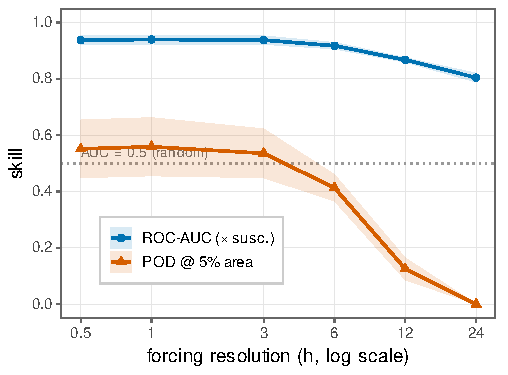
\includegraphics[width=0.6\linewidth]{figs/fig_synthetic.pdf}
\caption{Controlled resolution experiment (mean over 20 random realisations; bands
$\pm1$ sd). Synthetic half-hourly rainfall fields, aggregated to coarser resolution
(log axis) under a fixed I--D engine (calibrated regional $a^\star=5.5$) and 24\,h
maximum duration, scored against labels from an \emph{independent} pore-pressure
store rather than from the I--D rule itself. Stratifying by failure mechanism is
what reveals the effect: the operational catch rate on \textbf{burst-driven}
failures (orange) collapses from 0.46 to 0.00, while \textbf{accumulation-driven}
failures (green) are caught at ${\approx}0.42$ at every resolution. The pooled
susceptibility-weighted AUC (blue) barely moves ($0.93\to0.91$) precisely because it
averages the two, which is why a pooled score hides the phenomenon. Daily
aggregation (intensity capped at total$/24$\,h) destroys the sub-daily triggering
route specifically, with the model and terrain held fixed.}
\label{fig:synthetic}
\end{figure}

\subsection{Resolution head-to-head}
\label{sec:headtohead}

The previous null motivates a controlled comparison of forcing resolution on the
same storm core (Atacama, 24--26 March 2015; the IMERG event-total maximum at
lon $-70.45$, lat $-27.15$), with the identical I--D engine
(Table~\ref{tab:headtohead}). The core is selected \emph{conditional on the known
event}, so this is a triggering-timing comparison, can each product cross the curve,
and when, not a discrimination test; discrimination is the business of the
distributed backtest (Section~5.2) and the controlled experiment
(Section~\ref{sec:synthetic}). Throughout this section and the next we use the
regional intercept $a^\star=5.5$\,mm\,h$^{-1}$ calibrated in Section~\ref{sec:lumped}, the only I--D curve fitted to data in this work, and not a value chosen to make the comparison work. Section~\ref{sec:intercept} shows the conclusion does
not rest on that choice. With a daily value the finest resolvable duration is
24\,h, so the maximum resolvable mean intensity is (daily total)$/24$\,h: CR2MET
sees 30.1\,mm spread to 0.66\,mm\,h$^{-1}$, an exceedance of at most 0.45
(the calibrated regional $a^\star=5.5$) or 0.17 (Caine), the daily product \textbf{structurally cannot
trigger}, for this storm's daily depth (its wettest day is 15.9\,mm); a larger daily total does cross the curve, as the 7 Maipo days of Section~\ref{sec:lumped} show. The same storm core in half-hourly IMERG peaks at
40\,mm\,h$^{-1}$; the I--D threshold is crossed at 04:30 UTC on 24 March
($E\approx9$), hours before the documented flows (Fig.~\ref{fig:leadtime}).
Higher-resolution forcing overcomes the limit with no change to the engine.

This comparison, however, moves \emph{two} things at once. The two products also
disagree on magnitude (IMERG 108\,mm vs CR2MET 30\,mm at this
core); IMERG is known to overestimate in arid convective regimes while CR2MET,
gauge-blended over a near-ungauged zone, likely underestimates, so the true
total lies between. A CR2MET-daily vs IMERG-half-hourly contrast therefore
confounds the product with its resolution, Section~\ref{sec:singlefactor} separates the two, and its result qualifies this one: at \emph{this} event the product, not the resolution, decides detection.
What survives the separation unchanged is the timing: no daily product, whatever
its magnitude, can place the crossing at 04:30. The purely
arithmetic part of the argument is also independent of the magnitude dispute:
even taking CR2MET's own 30\,mm total, spreading it over 24\,h yields a
mean intensity far below the I--D curve, so a daily product cannot trigger
regardless of which magnitude is correct.

\begin{table}[ht]
\centering
\caption{CR2MET daily vs.\ GPM IMERG half-hourly at the Atacama storm core (same I--D engine).}
\label{tab:headtohead}
\begin{tabular}{@{}lcc@{}}
\toprule
 & CR2MET daily ($\sim$5\,km) & IMERG $\frac{1}{2}$-hourly ($\sim$10\,km) \\
\midrule
event total (24--26 March, core cell) & 30.1\,mm & 108.5\,mm \\
wettest day / half-hour & 15.9\,mm & 20.0\,mm \\
finest resolvable duration & 24\,h & 0.5\,h \\
max resolvable intensity (wettest step$/$duration) & 0.66\,mm\,h$^{-1}$ & 40.0\,mm\,h$^{-1}$ \\
I--D ($a^\star=5.5$) & no alert ($E\leq0.45$) & alert 24-Mar 04:30 ($E\approx9$) \\
\bottomrule
\end{tabular}
\end{table}

\begin{figure}[t]
\centering
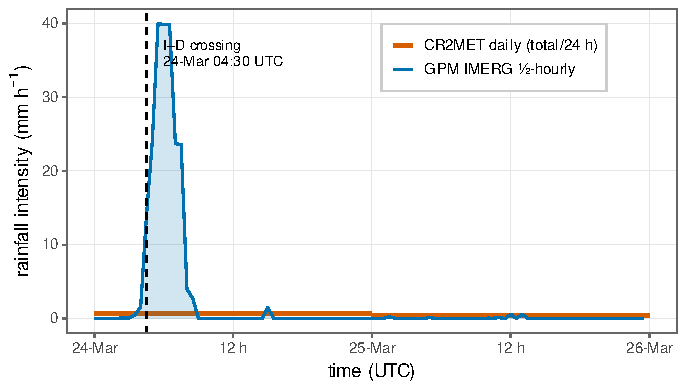
\includegraphics[width=0.78\linewidth]{figs/fig3_leadtime.pdf}
\caption{Forcing resolution at the Atacama storm core (24--26 March 2015). The
GPM IMERG half-hourly intensity (blue) peaks at 40\,mm\,h$^{-1}$ and crosses the
I--D curve at 04:30 UTC on 24 March; the same rainfall seen by a daily product
(CR2MET, orange: total$/24$\,h) is a flat 0.66\,mm\,h$^{-1}$ on the wettest day (and lower on the others) that never
reaches the curve. The daily product structurally cannot resolve the
triggering burst.}
\label{fig:leadtime}
\end{figure}

\subsection{Multi-event sub-daily lead time}
\label{sec:multievent}

The sub-daily result generalises across three dated debris-flow events in opposite
climates (Table~\ref{tab:multievent}). In all three the half-hourly I--D crossing
lands on or just before the documented day. For the Caj\'on del Maipo summer
convective burst, the same rainfall aggregated to daily \textbf{never triggers}, only
sub-daily resolution detects it --- note that this column already holds the product
fixed, since it aggregates the same IMERG series, which is the comparison
Section~\ref{sec:singlefactor} generalises. The inventory provides no event onset \emph{hour},
so these are not formal lead-time skill scores but a demonstration that sub-daily
forcing resolves the threshold-crossing time that daily forcing cannot.

As a spatial false-alarm check, we ran the identical per-cell I--D trigger over each
event's full IMERG scene. The documented storm core is in every case the most
extreme cell (96.7--100th percentile of peak exceedance), but the trigger crosses
the curve over a broad footprint, 30\,\% of the Atacama scene, 6\,\% at Caj\'on del
Maipo, and the entire (small, frontal) Villa Santa Luc\'ia box, so the crossing is
not spatially sparse within these storm-centred scenes. This locates the \emph{peak}
correctly but is \emph{not} a low false-alarm rate, and because the box is
event-centred by construction a high crossing fraction is expected. A genuine
discrimination estimate needs the off-event crossing frequency at these cores, a
multi-year sub-daily record on days \emph{without} a documented flow, which the
present event-window granules do not provide. The sub-daily results are therefore
triggering-timing demonstrations, not skill scores; assembling that multi-year
sub-daily record is, with a day-resolution inventory (Section~7), the key remaining
validation step.

\begin{table}[ht]
\centering
\caption{Sub-daily I--D crossing across three events (GPM IMERG half-hourly, storm
core, calibrated regional $a^\star=5.5$).}
\label{tab:multievent}
\begin{tabular}{@{}llcccc@{}}
\toprule
Event & Climate & Total & Peak 1\,h & Crossing (UTC) & Daily fires? \\
\midrule
Atacama/Copiap\'o & arid, convective & 108\,mm & 40\,mm\,h$^{-1}$ & 24-Mar 04:30 & yes \\
Caj\'on del Maipo & Andes, summer & 28\,mm & 5\,mm\,h$^{-1}$ & 25-Feb 17:30 & \textbf{no} \\
Villa Santa Luc\'ia & humid, frontal & 83\,mm & 17\,mm\,h$^{-1}$ & 15-Dec 15:30 & yes \\
\bottomrule
\end{tabular}
\end{table}

\subsection{Separating the product from its resolution}
\label{sec:singlefactor}

The head-to-head of Section~\ref{sec:headtohead} varies two things at once. CR2MET
daily and IMERG half-hourly differ both in temporal resolution and in the rainfall
product itself, and at these storm cores the two products disagree by up to a
factor of four in event total. Attributing the whole difference to resolution is
therefore unsound. We separate the factors by inserting the missing cell of the
design: the \emph{same} IMERG series aggregated to 24\,h. Each adjacent comparison
then moves exactly one factor,
\begin{center}
A. CR2MET daily $\;\xrightarrow{\text{product}}\;$ B. IMERG aggregated to 24\,h
$\;\xrightarrow{\text{resolution}}\;$ C. IMERG half-hourly,
\end{center}
and because exceedance is multiplicative in intensity the total ratio factorises
exactly, $E_C/E_A = (E_B/E_A)\cdot(E_C/E_B)$. To keep the test conservative, CR2MET
is read as the \emph{maximum} over its cells inside the IMERG pixel (giving the
daily product its best shot at the storm), and all three configurations see the same
event window and the same engine.

The outcome (Table~\ref{tab:singlefactor}) is more discriminating than the
head-to-head suggested, and it revises how that comparison should be read. At
Atacama the resolution factor is substantial ($\times3.2$) but the \emph{product}
factor is twice as large ($\times6.2$), and it is the product that flips detection:
IMERG aggregated to daily already crosses the curve ($E=2.8$). The claim that
supports the sub-daily case at this event is thus about timing, not detection ---
the daily series marks the day, only the half-hourly one places the crossing at
04:30. At Villa Santa Luc\'ia neither factor flips anything: CR2MET daily already
triggers ($E=1.6$), and resolution again buys timing alone. Only at Caj\'on del
Maipo does resolution flip detection with the product held fixed
($E=0.45\to1.23$), and there the product factor does not ($E=0.18\to0.45$, still
below the curve).

So of three events, resolution changes the \emph{detection} in one, and in that one the burst is short and weak, which is the regime the aggregation argument predicts. In all three it changes the \emph{timing}, which no daily product can
supply at any magnitude. We state the distinction plainly because the two claims
have different strengths: sub-daily forcing yields intra-day lead time generally,
whereas it rescues detection specifically for short bursts, and a case like
Atacama, where a daily product with the right magnitude would have fired anyway, is
not evidence for the second claim. The controlled experiment of
Section~\ref{sec:synthetic}, where the product is fixed by construction and only
resolution varies, is what isolates the detection effect at scale.

\begin{table}[ht]
\centering
\caption{Single-factor decomposition at each storm core: the product factor
(A$\to$B) and the resolution factor (B$\to$C) on the peak I--D exceedance $E$
($a^\star=5.5$). Bold marks the step that flips detection ($E$ crossing 1). The
CR2MET row (A) is the maximum over the CR2MET cells inside the IMERG pixel over
the window $D$ of the decomposition, so its total (26.8\,mm at Atacama) is not the
three-day core-cell total of Table~\ref{tab:headtohead} (30.1\,mm).}
\label{tab:singlefactor}
\small
\begin{tabular}{@{}llccccc@{}}
\toprule
Event & Configuration & Total & $I_{\max}$ & $D$ & $E$ & Fires? \\
 & & (mm) & (mm\,h$^{-1}$) & (h) & & \\
\midrule
\multirow{3}{*}{Atacama/Copiap\'o}
 & A. CR2MET daily         & 26.8 & 0.55 & 48 & 0.45 & no \\
 & B. IMERG at 24\,h       & 108.5 & 4.48 & 24 & \textbf{2.82} & \textbf{yes} \\
 & C. IMERG half-hourly    & 108.5 & 31.81 & 3 & 8.88 & yes \\
\multicolumn{7}{@{}l}{\quad\emph{product} $\times6.2$ $\cdot$ \emph{resolution} $\times3.2$ --- \emph{product flips detection; resolution adds timing}} \\
\midrule
\multirow{3}{*}{Caj\'on del Maipo}
 & A. CR2MET daily         & 6.9 & 0.29 & 24 & 0.18 & no \\
 & B. IMERG at 24\,h       & 27.5 & 0.54 & 48 & 0.45 & no \\
 & C. IMERG half-hourly    & 27.5 & 4.41 & 3 & \textbf{1.23} & \textbf{yes} \\
\multicolumn{7}{@{}l}{\quad\emph{product} $\times2.5$ $\cdot$ \emph{resolution} $\times2.8$ --- \emph{resolution flips detection, product alone does not}} \\
\midrule
\multirow{3}{*}{Villa Santa Luc\'ia}
 & A. CR2MET daily         & 72.2 & 2.53 & 24 & 1.59 & yes \\
 & B. IMERG at 24\,h       & 83.1 & 2.73 & 24 & 1.72 & yes \\
 & C. IMERG half-hourly    & 83.1 & 12.43 & 3 & 3.47 & yes \\
\multicolumn{7}{@{}l}{\quad\emph{product} $\times1.1$ $\cdot$ \emph{resolution} $\times2.0$ --- \emph{neither flips detection; resolution adds timing}} \\
\bottomrule
\end{tabular}
\end{table}

\subsection{The sub-daily result does not rest on the chosen intercept}
\label{sec:intercept}

Sections~\ref{sec:headtohead}--\ref{sec:multievent} apply one I--D curve, and a
sceptical reader may reasonably ask whether the conclusion is an artefact of that
choice: a low enough intercept makes any storm trigger, and a high enough one makes
none. We remove the choice in two ways.

First, the intercept can be \emph{measured} rather than chosen. Because exceedance
scales exactly as $1/a$ --- $E(a)=I\,D^{b}/a$, so $E(a)=(a_0/a)\,E(a_0)$ --- and the
window that maximises it is therefore the same for every $a$, each event has a
well-defined \emph{critical intercept}
\begin{equation}
a_\mathrm{crit} \;=\; \max_{t,m}\; I(t,m)\,D(m)^{b},
\label{eq:acrit}
\end{equation}
the highest intercept at which that event still crosses the curve. It is a property
of the observed rainfall and of $b$, not of the analyst. Computing it on the
half-hourly series and on the same series aggregated to daily yields two values,
and the interval between them,
$a_\mathrm{crit}(\text{daily}) < a \leq a_\mathrm{crit}(\text{half-hourly})$, is the
band of thresholds in which \emph{resolution alone} decides detection. That band
spans a factor of 2.0--3.2 in $a$ at all three events (Table~\ref{tab:intercept}),
and the calibrated $a^\star=5.5$ falls inside it at Caj\'on del Maipo --- which is
why the daily product misses that event at the intercept the paper calibrates
independently, in the Maipo backtest, and not at one tuned for this comparison.

Second, and without selecting any intercept at all, we re-ran the 35 published
power laws of \citet{guzzetti2007} --- each with its own $(a,b)$, unchanged ---
over each event at both resolutions. Resolution flips the outcome (sub-daily fires,
daily does not) for 8 of 35 curves at Atacama, 8 of 35 at Villa Santa Luc\'ia, and 2
of 35 at Caj\'on del Maipo. The Caj\'on del Maipo figure also shows the limit of that event: it is a weak burst (28\,mm, 5\,mm\,h$^{-1}$ peak) that only 4
of the 35 published curves detect at \emph{any} resolution, so while the
resolution effect there is real, it is demonstrated on an event near the detection
floor of the literature. At the two stronger events, where most published curves do
fire, the resolution effect is carried by roughly a quarter of the ensemble. Both
analyses are reproduced by the \texttt{intercept\_sensitivity} example.

Two caveats bound this. Applying $a^\star$, fitted in the R\'io Maipo, to storms in
the Atacama and in Patagonia is a transfer well outside its calibration region, and we make no claim that 5.5\,mm\,h$^{-1}$ is the right regional curve for either. Table~\ref{tab:intercept} shows that the resolution result survives whatever intercept one adopts within a broad band, so no such claim is needed. And $b$ is held at 0.39 throughout: the critical intercept of
Eq.~\ref{eq:acrit} is defined for a given exponent, and the published-curve
ensemble, which varies $b$ from 0.19 to 1.50, is what covers that dimension.

\begin{table}[ht]
\centering
\caption{Critical I--D intercept $a_\mathrm{crit}$ (Eq.~\ref{eq:acrit}, $b=0.39$) per
event and forcing resolution, and the band of intercepts in which resolution alone
decides detection.}
\label{tab:intercept}
\begin{tabular}{@{}lcccc@{}}
\toprule
Event & $a_\mathrm{crit}$ half-hourly & $a_\mathrm{crit}$ daily & ratio & resolution decides for \\
 & (mm\,h$^{-1}$) & (mm\,h$^{-1}$) & & (mm\,h$^{-1}$) \\
\midrule
Atacama/Copiap\'o & 48.8 & 15.5 & 3.2$\times$ & $15.5 < a \leq 48.8$ \\
Caj\'on del Maipo & 6.8 & 2.5 & 2.8$\times$ & $2.5 < a \leq 6.8$ \hfill ($\ni a^\star$) \\
Villa Santa Luc\'ia & 19.1 & 9.4 & 2.0$\times$ & $9.4 < a \leq 19.1$ \\
\bottomrule
\end{tabular}
\end{table}

\paragraph{Sensitivity to the remaining hyperparameters}
The exponent $b$, the maximum I--D duration, the logistic steepness $k$ and the alert level are held fixed elsewhere in the paper. Moving each one at a time on the lumped backtest (Table~\ref{tab:oat}) shows that the \emph{optimum} moves and the \emph{skill at the optimum} does not: re-calibrating $a^\star$ by maximum CSI under $b=0.19$, $0.565$ (the median of the 35 published curves) and $0.78$ gives $a^\star$ of 2.5, 13.5 and 13.0\,mm\,h$^{-1}$ with CSI 0.080, 0.082 and 0.066 against 0.077 at the paper's setting, and every (steepness, level) pair, which enters only through the exceedance at which the hazard crosses the level, $E_\mathrm{thr}=1+\ln[L/(1-L)]/k$, leaves CSI within 0.071--0.079. At the paper's fixed $a^\star=5.5$ the scores do move with $b$ (POD 0.11 at $b=0.19$, 0.89 at $b=0.78$), which is the statement that $a$ and $b$ are not separately identified by a monthly contingency. At the three storm cores the half-hourly exceedance changes little with $b$ but the daily one changes a lot, because the daily window is 24\,h and $D^b$ grows with $b$: at $b=0.78$ the daily series at Atacama and Villa Santa Luc\'ia crosses comfortably and the Caj\'on del Maipo daily value reaches 1.47, so the ``daily does not fire'' column of Table~\ref{tab:singlefactor} is the $b$-sensitive one and holds for exponents up to about 0.6. Rank-based scores are invariant to $k$ by construction (Section~4.2) and were not re-run; the 30\,m-to-5\,km aggregation operator of Section~5.2 (the 90th percentile per cell) was not varied, which remains a gap.

\begin{table}[ht]
\centering
\small
\caption{One-at-a-time sensitivity of the lumped Maipo backtest ($\pm1$ month) and of the storm-core exceedances. Left: the max-CSI intercept re-calibrated under each setting, with POD/FAR/CSI at that optimum and at the paper's fixed $a^\star=5.5$. Right: peak exceedance $E$ at $a^\star=5.5$ for the half-hourly and the daily series of each core (24\,h maximum window), which crosses the curve when $E\geq1$.}
\label{tab:oat}
\begin{tabular}{@{}lcccc@{}}
\toprule
Setting & $a^\star$ & POD / FAR / CSI at $a^\star$ & POD / FAR / CSI at 5.5 & \\
\midrule
Paper: $b$ 0.39, $m_{\max}$ 7\,d, $k$ 4, level 0.5 & 5.5 & 0.53 / 0.92 / 0.077 & 0.53 / 0.92 / 0.077 & \\
$b=0.19$ & 2.5 & 0.58 / 0.91 / 0.080 & 0.11 / 0.94 / 0.041 & \\
$b=0.565$ & 13.5 & 0.47 / 0.91 / 0.082 & 0.63 / 0.94 / 0.056 & \\
$b=0.78$ & 13.0 & 0.74 / 0.93 / 0.066 & 0.89 / 0.95 / 0.053 & \\
$m_{\max}=1$\,d & 4.5 & 0.53 / 0.92 / 0.071 & 0.42 / 0.93 / 0.067 & \\
$m_{\max}=3$\,d & 4.5 & 0.58 / 0.92 / 0.075 & 0.47 / 0.92 / 0.071 & \\
$k$ 4, level 0.4 ($E_\mathrm{thr}$ 0.90) & 7.0 & 0.47 / 0.91 / 0.078 & 0.53 / 0.92 / 0.072 & \\
$k$ 4, level 0.6 ($E_\mathrm{thr}$ 1.10) & 5.0 & 0.53 / 0.92 / 0.077 & 0.47 / 0.92 / 0.075 & \\
$k$ 2, level 0.6 ($E_\mathrm{thr}$ 1.20) & 4.0 & 0.58 / 0.92 / 0.079 & 0.42 / 0.92 / 0.072 & \\
$k$ 8, level 0.6 ($E_\mathrm{thr}$ 1.05) & 6.0 & 0.47 / 0.91 / 0.078 & 0.47 / 0.92 / 0.072 & \\
\midrule
Core $E$ (half-hourly / daily) & Atacama & Caj\'on del Maipo & Villa Santa Luc\'ia & \\
$b=0.19$ & 7.83 / 1.49 & 1.06 / 0.23 & 3.07 / 0.91 & \\
$b=0.39$ (paper) & 8.88 / 2.82 & 1.23 / 0.43 & 3.47 / 1.72 & \\
$b=0.565$ & 10.80 / 4.91 & 1.51 / 0.74 & 4.35 / 2.99 & \\
$b=0.78$ & 14.14 / 9.73 & 2.00 / 1.47 & 7.46 / 5.93 & \\
\bottomrule
\end{tabular}
\end{table}

\subsection{Flood path: a routed-discharge check against observed streamflow}

To exercise the discharge trigger we run GR4J \citep{perrin2003} on the CAMELS-CL
R\'io Itata catchment (gauge 8123001, 1979--2016) and validate it against
\emph{observed} daily streamflow. Unlike the month-dated landslide inventory,
observed streamflow is daily, so this is a genuine day-resolution verification.
GR4J is calibrated by random search on the training period (years before 2003,
maximising Kling--Gupta efficiency \citep{gupta2009}) and evaluated out of sample on 2003--2016; it
reproduces the observed hydrograph well (KGE 0.85 train, 0.74 test; NSE 0.70 / 0.60).
Defining an observed flood as a day whose observed discharge exceeds its 98th
training percentile (21.7\,mm\,day$^{-1}$), the engine's discharge-exceedance hazard,
driven by the \emph{simulated} hydrograph, discriminates the 60 observed flood days of the test period
with ROC-AUC 0.896 [0.826, 0.972] (year-block bootstrap, 2\,000 resamples); at a fixed alert level (simulated $Q$ above the
98th training percentile, 23.2\,mm\,day$^{-1}$) it scores POD 0.30, FAR 0.42 and
CSI 0.25 against a 1.2\,\% flood base rate. Two things must be said about that
number. First, it measures the wrapped model, not the engine: with one lumped
catchment the exposure factor is a constant and the discharge trigger is monotone
in $Q$, so by the invariance of Section~4.2 the hazard ranks days exactly as the
simulated hydrograph does, and the run is driven by observed rainfall, so its lead
time is zero. Second, it does not beat model-free baselines on the same days:
yesterday's observed discharge (persistence) scores 0.946 [0.912, 0.966], the
observed 3-day rainfall sum 0.942 [0.883, 0.987], and the observed 1-day rainfall
0.824 [0.777, 0.884]. The exact-attribution facility
decomposes each alert into its exposure and discharge factors, but the flood path as
exercised here is a check that the routed-discharge trigger behaves, not a validated
nowcast.

What the check does establish is the resolution argument seen from the other side. Discharge routing
\emph{integrates} rainfall over the catchment, supplying the temporal accumulation
that a sub-daily I--D trigger must otherwise resolve in the rainfall itself; a daily
forcing that cannot trigger a convective-burst landslide
(Section~\ref{sec:singlefactor}) is therefore adequate for a routed-discharge flood, so adequate that a 3-day rainfall sum already discriminates flood days. Attainable skill
tracks the forcing resolution \emph{relative to the process}: daily suffices where
routing integrates, and fails where triggering is sub-daily.

\subsection{Architecture extensibility}

Beyond the two validated paths above, the engine ships further adapters that
exercise the \emph{interface} and make no hazard claim: none of them is a validated prediction. A snowmelt provider supplies rain-plus-melt runoff per cell by wrapping a distributed snowmelt model, which matters in the Andes because mountain snowmelt timing itself shifts under warming \citep{musselman2017}. An InSAR provider turns a
line-of-sight velocity field into a duration-independent deformation trigger that
fuses with rainfall by noisy-OR, so a slope already creeping
($|v|>v_{\mathrm{crit}}$) can cross the alert level under rain that alone would not trigger. An agent-based debris-flow model, run on demand from an alert, returns
a runout footprint onto which the coarse probability is concentrated, the landslide analogue of the flood coupling of Section~2.5. A wildfire-spread model couples the other way, as a one-way cascade in which a simulated burn scar amplifies the
static susceptibility, so a subsequent rainfall nowcast sees the elevated post-fire
debris-flow hazard the scar is known to carry \citep{cannon2008}. Each is a runnable example. Their
purpose here is to show that a new forcing, a new trigger family and a new
physical-refinement model each plug in through the same \texttt{Forcing} and
\texttt{Trigger} interfaces \emph{without touching the hazard logic}; their
predictive skill rests on the wrapped models and their own validation, and is not
claimed here. The results this paper stands on are the resolution diagnosis
(Section~\ref{sec:synthetic}), the routed-discharge check (Section~5.8, which measures GR4J, not the engine) and the on-demand
coupling's compute saving (Section~2.5).

\section{Discussion}

The headline is a methods result obtained \emph{because} the engine holds the
model fixed while the forcing varies. \textbf{What resolution buys.}
Distributing daily rainfall and adding a real susceptibility raster does not lift
discrimination above chance, yet the identical trigger on sub-daily forcing
resolves the threshold crossing to within hours. The binding constraint on
\emph{timing} is therefore the resolution of the forcing, not the susceptibility model or the
threshold logic; on \emph{detection} the evidence is narrower, as the rest of this paragraph sets out, and where failures are antecedent-controlled the trigger itself is the ceiling (Table~\ref{tab:sweep}). This is intuitive once stated (with a daily value the maximum
resolvable intensity is total$/24$\,h, so short, intense, convective bursts are
smeared below any I--D curve), and the threshold literature has measured its first-order effect: coarse temporal resolution biases fitted thresholds downward \citep{marra2019,gariano2020}, and rainfall-estimation uncertainty and spatial aggregation shift them \citep{nikolopoulos2014,marra2017}. Those studies refit the threshold to each dataset; what is rarely isolated is the effect of resolution under one fixed trigger, separated from the product, which is what the one-factor design does. Isolating it
demands care in the other direction too: comparing a daily gauge-blended product
against a half-hourly satellite one varies the product as well as its resolution,
and Section~\ref{sec:singlefactor} shows the two factors can point to different
conclusions at the same event --- at Atacama the product is what decides detection,
and resolution only the timing. We therefore keep the two claims separate
throughout: sub-daily forcing buys intra-day timing in general, and buys detection
where the triggering burst is short. The
controlled experiment (Section~\ref{sec:synthetic}) makes the mechanism explicit on
a target whose labels come from an independent physical process: with the model and
terrain held fixed, aggregation drives the catch rate on burst-driven failures to
zero while sparing accumulation-driven ones entirely, so the real-data null is consistent with a resolution limit on burst-driven failures, which it cannot establish on its own (Section~5.2), and the controlled experiment measures the mechanism rather than the field skill. It also shows why a pooled skill score can conceal this, by averaging
the two populations. The practical corollary is that an I--D nowcast is only as good as its
rainfall's temporal resolution; effort spent on susceptibility sophistication is
wasted where the forcing is daily. The flood path makes the same point from the other side: where discharge routing integrates the rainfall, daily
forcing is adequate, and so adequate that the GR4J-driven hazard (ROC-AUC 0.90, Section~5.8) is matched by a
3-day rainfall sum and by persistence (0.94--0.95), which is a statement about the process, not a validated nowcast. Skill thus tracks forcing resolution \emph{relative to
the triggering process}, not resolution in the abstract, a daily product that is
useless for convective-burst landslides is sufficient for routed floods.

\textbf{The product ceiling, observed live.} The first weeks of shadow operation
(limitation~(iii)) add a case the hindcasts could not: two convective bursts of
twenty to sixty minutes, one of which caused a debris flow, that both half-hourly
satellite products under-recorded by an order of magnitude at Las Condes and by
enough to stay below any I--D curve at Curacaut\'in, while a rain gauge 7\,km
away and the geostationary lightning mapper did not. Half-hourly resolution is
necessary but not sufficient: at the scale of a single convective cell the
satellite rainfall estimate, not the time step, is the binding constraint, and
the low-latency sensor that resolves the burst is the one that does not measure
rain. For burst-driven landslides the forcing interface therefore has to admit
dense in-situ networks and convective proxies alongside satellite QPE, which is
exactly the swap the design was built to make cheap.

The same arithmetic bites on a second, less obvious surface: the
\emph{climatological reference} against which an event is judged anomalous. For
the dated 2026 event replayed in limitation~(iii) (Coelemu, \~Nuble, 31 July 2026) we compared the observed half-hourly
accumulation at the affected commune against that commune's own winter
climatology (CR2MET v2.5, May--September 1991--2020; \citealp{boisier2018cr2met}). At a 24\,h window the event sits
at the 99.96th percentile, equalled twice in thirty winters ($\approx$1-in-15).
Aggregated to five days the identical event falls to the 97th percentile and is
equalled 127 times, roughly five times per winter, because it concentrated 87\,\%
of its five-day total into two days. A rarity statistic computed on a window
wider than the triggering burst therefore reports a routine event where a
1-in-15-winter one occurred. The consequence is operational. Anomaly- or return-period-based triggers are a common alternative to fixed I--D curves, and they inherit the resolution ceiling through the reference climatology even when the
forcing itself is sub-daily, which is a failure mode the forcing-side diagnosis
alone does not expose.

\textbf{The inventory ceiling.} A second, independent ceiling is the validation
target. The inventory is dated to $\sim$month and is incomplete, echoing a
broader finding, from synthetic experiments, that uncertain identification of the
triggering rainfall episode itself distorts threshold assessment, generally biasing
thresholds low, with an effect that grows once dating errors exceed one day
\citep{peres2018}. Month-level
dating alone accounts for a large fraction of apparent misses
(Table~\ref{tab:lumped}), and incompleteness makes per-cell FAR uninformative.
Credible discrimination and true lead-time skill require a day- or hour-resolution
inventory, or event-segmented rainfall, a data problem, not a software one, and
the single largest unlock for future validation.

\textbf{The architecture as enabler.} That both diagnoses were even possible rests
on the forcing-agnostic design: swapping CR2MET daily for IMERG half-hourly, or
adding a deformation trigger, requires no change to the hazard logic. The same
interface lets the engine act as the downstream integrator of a family of process
models, and the one-way on-demand coupling keeps the expensive physics confined to
alerted areas. It occupies a different design point from existing tools and does not replace them. Operational nowcasts such as LHASA couple a static susceptibility map with a
specific rainfall product (IMERG) and trigger, as a global monolithic chain
\citep{kirschbaum2018}, and its data-driven successor replaces that map with
explanatory variables inside the same fixed chain \citep{stanley2021}; threshold
calculators such as CTRL-T \citep{melillo2018} automate the estimation of regional
cumulated-rainfall--duration (E--D) thresholds from rain-gauge records and
landslide catalogues.
nowcast is complementary: it makes the forcing, the trigger and the
physical-refinement model \emph{independently swappable} behind one interface, and that is what let us hold the model fixed and vary the forcing resolution. It is
an experimental and integrating substrate, not a calibrated operational product, and
an operational chain like LHASA is the kind of system its outputs would feed or be
benchmarked against.

\section{Limitations and future work}
\label{sec:limits}

Six things are still missing from the engine. (i) The raw hazard
is a bounded \emph{index}; the engine ships isotonic calibration \citep{niculescumizil2005} that maps it to a
probability with reliability diagnostics (Brier score and skill \citep{brier1950}, Wilson intervals \citep{wilson1927},
expected calibration error). Fitting it on the real distributed Maipo backtest
(odd years $\to$ even) collapses the calibrated probability to climatology (Brier
skill $-3.4$ for the raw index $\to -0.003$ calibrated; expected calibration error $0.080\to0.003$), which confirms that the daily index carries no skill to calibrate, consistent with the Section~5.2 null. Validating the calibration where
skill is present (routed discharge, sub-daily forcing) remains future work.
(ii) Trigger parameters are calibrated
minimally; a formal calibration with uncertainty, for which the sibling
rainfall--runoff engine already provides a DDS \citep{tolson2007} optimiser pattern, is future work.
We benchmark discrimination against supervised baselines (Section~5.2) and against
the full ensemble of 35 published I--D thresholds (Section~5.1), but a formal
calibration with uncertainty against an \emph{operational} early-warning system
remains future work. (iii) The engine includes a streaming nowcast that ingests
forcing step by step and emits alerts online (bit-identical to the batch engine).
A live multi-feed ingestion chain is wired (half-hourly GPM IMERG Early NRT,
GOES-East QPE and in-situ rain gauges, fused by noisy-OR), and we replayed one dated
2026 landslide event (Coelemu, \~Nuble Region, 31 July 2026) through it end to end. The engine placed the affected
commune in alert for a ten-hour window on the day of the flows, crossing the
threshold at 01:30 local time. But the alert covered roughly 40\,\% of the domain at
its peak: at $0.1^{\circ}$ the run identifies the region and the timing, not the
commune, so this is a consistency check rather than an operational skill
estimate. Since October 2026 the chain has run in shadow mode over three domains
(Atacama, Santiago and the Araucan\'ia), and its first weeks already sharpen the
forcing diagnosis of the Discussion. On 8 October a one-hour convective burst on
the Andean piedmont of Santiago produced a debris flow; a gauge 7\,km from the
site recorded 12.6\,mm in four hours, 8.2 of them in the hour before the flow,
while IMERG Early and GOES QPE recorded 0.37 and 1.66\,mm in the same cell. On
satellite forcing alone the hazard in the burn scar stayed below 0.05 with either
intercept; the gauge feed with the regional intercept crossed the alert level
(0.29 against 0.267) at the hour of the flow, with no lead. On 12 October the
Santiago domain produced its first real-time crossing, again sustained only by
the gauge feed (9.4\,mm in the cell against 0.3 and 0.1\,mm from the two satellite
products); no damage has been reported and it is not yet classified. The same
afternoon a twenty-minute hail storm flooded 21 houses in Curacaut\'in, 600\,km
to the south, where no gauge exists within 45\,km: GOES QPE saw 3.5\,mm in the
city cell, and IMERG Early did resolve the cell (3.6\,mm in 30\,min), so that the
hazard crossed one hour after the event, but that product is published some four
hours late. In both convective cases the geostationary lightning mapper on the
same satellite \citep{goodman2013} registered the cell first: 233 flashes over
the piedmont with the peak thirty minutes before the Las Condes flow, and 118
flashes within 5\,km of Curacaut\'in from an hour before the flooding. The chain
now carries lightning as a diagnostic rather than a forcing, weighs a single-feed
crossing by which feed sustains it, and freezes the evidence of every alert
automatically. Three events in five days, reported by the press rather than by an
inventory, do not constitute a skill estimate, and the false-alarm rate of the
regional intercept is still being measured; the shadow season remains the
necessary step, and the validation reported in Sections~5.1--5.8 is hindcast
throughout.
(iv) Antecedent soil moisture is captured only implicitly through long rolling
windows, not as an explicit state, and the controlled experiment measures what that costs: when failures are controlled by a store that drains over days rather than hours, the I--D trigger catches under 10\,\% of them at any resolution (Table~\ref{tab:sweep}), so for antecedent-controlled landslides the model, not the forcing, is the ceiling, and a state trigger fed by the sibling rainfall--runoff store is the one-adapter change the architecture was built for. (v) The multi-trigger combination weights and
the deformation critical rate are not yet calibrated. (vi) The snowmelt, InSAR-deformation
and debris-flow-runout adapters (Section~5.9) exercise the architecture but are not
validated predictions; only the on-demand coupling's compute saving is quantified
(Section~2.5).
Addressing (i), (ii) and a day-resolution inventory would convert the present
diagnosis into a validated operational claim.

\section{Conclusions}

\texttt{nowcast} is an open, dependency-light Rust engine that turns static
susceptibility into a time-varying hazard through a single interchangeable forcing
interface and a composable trigger, with native providers for rainfall--runoff,
snowmelt, shallow-water inundation, agent-based debris-flow runout, a geospatial
substrate and InSAR deformation, and exact closed-form attribution of every alert.
Used as an experimental instrument over Chilean basins, it yields a diagnosis that, we argue, generalises: what sub-daily forcing buys an intensity--duration trigger is intra-day timing in every case and detection only for short bursts, while the magnitude error of the rainfall product, and in operation the sensor, bind elsewhere. A global I--D threshold is reached on 7 of 13\,880 days and never on a recorded event month. A calibrated regional threshold transfers split-sample but is not distinguishable from a seasonal null, and at daily resolution and distributed over the basin it does not discriminate event locations (AUC $\approx 0.48$). The identical trigger on half-hourly satellite forcing places
the threshold crossing at a timestamp hours ahead of the documented flows on the same day across three
climatically distinct events, and a single-factor decomposition separates what that
gain owes to the rainfall product from what it owes to its resolution, which turns
out to differ by event. The engine, its backtesting framework and all
examples are reproducible, and the architecture is designed so that
higher-resolution and better-measured forcing, the demonstrated path to timing and the diagnosed path to detection, can be plugged in
without touching the hazard logic.

\section*{Code and data availability}

The \texttt{nowcast} source (twelve Rust crates, including a command-line runner and
PyO3 Python bindings, plus thirty-six examples) and all data-extraction scripts
are openly available at \url{https://github.com/franciscoparrao/nowcast} under the
MIT or Apache-2.0 licence; a citable snapshot of the version used here (v0.2.0) is archived on
Zenodo at \url{https://doi.org/10.5281/zenodo.23198956} (concept DOI
\url{https://doi.org/10.5281/zenodo.22019137}, which always resolves to the
latest version). 

\paragraph{What the archived snapshot reproduces, and what it does not}
Reproducibility here is not uniform across the paper, and it would be misleading to
claim otherwise. \texttt{nowcast-core} has \emph{no} path dependencies: it builds
and tests offline with no system dependencies, and its 22 examples regenerate every
result in Sections~\ref{sec:lumped}--\ref{sec:intercept} --- the lumped and
distributed backtests and their null diagnostics, the published-threshold ensemble,
the controlled resolution experiment, the head-to-head, the multi-event lead times,
the single-factor decomposition and the intercept sensitivity --- from the archived
snapshot alone, given the derived input CSVs (regenerated by the extraction scripts
from the third-party datasets below), through \texttt{scripts/reproduce\_core.sh}.
The script is needed because Cargo resolves every member of a workspace before
building any of them, so a plain build at the snapshot root would already require
the sibling repositories; it builds the core in a workspace of its own and runs its
tests and the paper's examples. The provider crates are different: each wraps
a sibling engine of the author's Rust geohazard family through a \emph{path}
dependency to a repository outside this snapshot, so the flood path of
Section~5.8 (GR4J on CAMELS-CL Itata, ROC-AUC 0.90, in
\texttt{nowcast-rainflow}), the coupling demonstrations of Section~5.9 and the
command-line runner, which links the geospatial substrate, cannot be rebuilt from
the Zenodo record on its own; they require the sibling repositories checked out
alongside, which \texttt{scripts/check\_siblings.sh} verifies and the README
documents. Publishing the sibling engines as versioned registry crates would close
this gap and is the intended path; until then the scope of the archived artefact is the core engine and the resolution results, which is where the paper's
claims live. Input datasets are third-party and openly documented: CR2MET v2.5,
GPM IMERG Final v07 and Early NRT v07 (NASA GES DISC; the latter feeds the live
chain of limitation~(iii)), GOES-East ABI-L2-RRQPEF (NOAA, public AWS bucket),
CAMELS-CL
(\citealp{alvarez2018}; \url{https://doi.org/10.1594/PANGAEA.894885}) and the
SERNAGEOMIN inventory.

\paragraph{Software availability}
\emph{Name}: \texttt{nowcast}.
\emph{Developer}: Francisco Parra.
\emph{Contact}: see corresponding author.
\emph{Year first available}: 2026.
\emph{Hardware required}: any 64-bit machine; the experiments in this paper run on
a laptop (the full example suite in minutes; see Section~2.8 for timings).
\emph{Software required}: Rust 1.85 or later (stable; the 2024 edition) for the core engine, and 1.91
or later for the command-line runner, whose geospatial dependency declares it;
Python 3.9 or later with \texttt{maturin} for the optional bindings; R with
\texttt{ggplot2} to regenerate the figures; the data-extraction scripts need
\texttt{numpy}, \texttt{netCDF4}, \texttt{xarray} and \texttt{earthaccess}.
\emph{Program language}: Rust (with Python bindings via PyO3).
\emph{Program size}: approximately 17\,000 lines of Rust across twelve crates.
\emph{Availability and cost}: free and open source, MIT or Apache-2.0, at the
repository and Zenodo DOIs above.

\section*{Funding}

This work was supported by the Direcci\'on de Investigaci\'on Cient\'ifica y
Tecnol\'ogica (DICYT), Vicerrector\'ia de Investigaci\'on, Innovaci\'on y
Creaci\'on, Universidad de Santiago de Chile [project code
062619MC\_POSTDOC]. The funder had no role in study design, in the collection,
analysis and interpretation of data, in the writing of the report, or in the
decision to submit the article for publication.

\section*{Acknowledgements}

The author acknowledges Project 062619MC\_POSTDOC of the Vicerrector\'ia de
Investigaci\'on, Innovaci\'on y Creaci\'on, Universidad de Santiago de Chile.
The author also thanks the CR2 (Center for Climate and
Resilience Research) for CR2MET, NASA for GPM IMERG, and SERNAGEOMIN for the
landslide inventory.

\section*{Declaration of generative AI and AI-assisted technologies in the writing process}

During the preparation of this work the author used Anthropic Claude, a large
language model, to assist with drafting and editing the manuscript text and with
the software implementation and exploratory analysis. After using this tool the
author reviewed and edited the content as needed and takes full responsibility for
the content of the publication.

\section*{CRediT authorship contribution statement}

\textbf{Francisco Parra}: Conceptualization, Methodology, Software, Validation,
Formal analysis, Investigation, Data curation, Writing --- original draft,
Writing --- review \& editing, Visualization.

\section*{Declaration of competing interest}

The author declares that he has no known competing financial interests or
personal relationships that could have appeared to influence the work reported in
this paper.

\begin{thebibliography}{99}

\bibitem[Alvarez-Garreton et al.(2018)]{alvarez2018}
Alvarez-Garreton, C., et al., 2018. The CAMELS-CL dataset: catchment attributes
and meteorology for large sample studies, Chile dataset. Hydrol.\ Earth Syst.\
Sci.\ 22, 5817--5846. \url{https://doi.org/10.5194/hess-22-5817-2018}.

\bibitem[Andrews(2018)]{andrews2018}
Andrews, P.L., 2018. The Rothermel surface fire spread model and associated
developments: A comprehensive explanation. USDA Forest Service, Rocky Mountain
Research Station, RMRS-GTR-371. \url{https://doi.org/10.2737/rmrs-gtr-371}.

\bibitem[Audusse et al.(2004)]{audusse2004}
Audusse, E., Bouchut, F., Bristeau, M.-O., Klein, R., Perthame, B., 2004. A fast
and stable well-balanced scheme with hydrostatic reconstruction for shallow water
flows. SIAM J.\ Sci.\ Comput.\ 25 (6), 2050--2065.
\url{https://doi.org/10.1137/S1064827503431090}.

\bibitem[Berardino et al.(2002)]{berardino2002}
Berardino, P., Fornaro, G., Lanari, R., Sansosti, E., 2002. A new algorithm for
surface deformation monitoring based on small baseline differential SAR
interferograms. IEEE Trans.\ Geosci.\ Remote Sens.\ 40 (11), 2375--2383.
\url{https://doi.org/10.1109/tgrs.2002.803792}.

\bibitem[Bogaard and Greco(2018)]{bogaard2018}
Bogaard, T., Greco, R., 2018. Invited perspectives: Hydrological perspectives on
precipitation intensity--duration thresholds for landslide initiation: proposing
hydro-meteorological thresholds. Nat.\ Hazards Earth Syst.\ Sci.\ 18, 31--39.
\url{https://doi.org/10.5194/nhess-18-31-2018}.

\bibitem[Boisier et al.(2018a)]{boisier2018}
Boisier, J.P., Alvarez-Garreton, C., Cordero, R.R., et al., 2018a. Anthropogenic
drying in central-southern Chile evidenced by long-term observations and climate
model simulations. Elementa: Science of the Anthropocene 6.
\url{https://doi.org/10.1525/elementa.328}.

\bibitem[Boisier et al.(2018b)]{boisier2018cr2met}
Boisier, J.P., Alvarez-Garret\'on, C., Cepeda, J., Osses, A., V\'asquez, N.,
Rondanelli, R., 2018b. CR2MET: A high-resolution precipitation and temperature
dataset for hydroclimatic research in Chile. EGU General Assembly 2018.

\bibitem[Brunetti et al.(2018)]{brunetti2018}
Brunetti, M.T., Melillo, M., Peruccacci, S., Ciabatta, L., Brocca, L., 2018. How
far are we from the use of satellite rainfall products in landslide forecasting?
Remote Sens.\ Environ.\ 210, 65--75. \url{https://doi.org/10.1016/j.rse.2018.03.016}.

\bibitem[Brier(1950)]{brier1950}
Brier, G.W., 1950. Verification of forecasts expressed in terms of probability.
Mon.\ Weather Rev.\ 78 (1), 1--3.
\url{https://doi.org/10.1175/1520-0493(1950)078<0001:VOFEIT>2.0.CO;2}.

\bibitem[Caine(1980)]{caine1980}
Caine, N., 1980. The rainfall intensity--duration control of shallow landslides
and debris flows. Geogr.\ Ann.\ A 62, 23--27.
\url{https://doi.org/10.1080/04353676.1980.11879996}.

\bibitem[Cannon and DeGraff(2008)]{cannon2008}
Cannon, S.H., DeGraff, J., 2008. The increasing wildfire and post-fire
debris-flow threat in western USA, and implications for consequences of climate
change. In: Sassa, K., Canuti, P. (Eds.), Landslides -- Disaster Risk Reduction.
Springer, pp.\ 177--190. \url{https://doi.org/10.1007/978-3-540-69970-5_9}.

\bibitem[D'Ambrosio et al.(2003)]{dambrosio2003}
D'Ambrosio, D., Di Gregorio, S., Iovine, G., 2003. Simulating debris flows
through a hexagonal cellular automata model: SCIDDICA S3-hex. Nat.\ Hazards
Earth Syst.\ Sci.\ 3, 545--559. \url{https://doi.org/10.5194/nhess-3-545-2003}.

\bibitem[David et al.(2013)]{david2013}
David, O., Ascough, J.C., Lloyd, W., Green, T.R., Rojas, K.W., Leavesley, G.H.,
Ahuja, L.R., 2013. A software engineering perspective on environmental modeling
framework design: The Object Modeling System. Environ.\ Model.\ Softw.\ 39,
201--213. \url{https://doi.org/10.1016/j.envsoft.2012.03.006}.

\bibitem[Ferretti et al.(2001)]{ferretti2001}
Ferretti, A., Prati, C., Rocca, F., 2001. Permanent scatterers in SAR
interferometry. IEEE Trans.\ Geosci.\ Remote Sens.\ 39 (1), 8--20.
\url{https://doi.org/10.1109/36.898661}.

\bibitem[Finney(1998)]{finney1998}
Finney, M.A., 1998. FARSITE: Fire Area Simulator---model development and
evaluation. USDA Forest Service, Rocky Mountain Research Station, RMRS-RP-4.
\url{https://doi.org/10.2737/rmrs-rp-4}.

\bibitem[Friedman(2001)]{friedman2001}
Friedman, J.H., 2001. Greedy function approximation: A gradient boosting
machine. Ann.\ Stat.\ 29 (5), 1189--1232.
\url{https://doi.org/10.1214/aos/1013203451}.

\bibitem[Gariano and Guzzetti(2016)]{gariano2016}
Gariano, S.L., Guzzetti, F., 2016. Landslides in a changing climate.
Earth-Sci.\ Rev.\ 162, 227--252.
\url{https://doi.org/10.1016/j.earscirev.2016.08.011}.

\bibitem[Gariano et al.(2020)]{gariano2020}
Gariano, S.L., Melillo, M., Peruccacci, S., Brunetti, M.T., 2020. How much does
the rainfall temporal resolution affect rainfall thresholds for landslide
triggering? Nat.\ Hazards 100 (2), 655--670.
\url{https://doi.org/10.1007/s11069-019-03830-x}.

\bibitem[Garreaud et al.(2020)]{garreaud2019}
Garreaud, R.D., Boisier, J.P., Rondanelli, R., Montecinos, A., Sep\'ulveda, H.H.,
Veloso-Aguila, D., 2020. The Central Chile Mega Drought (2010--2018): a climate
dynamics perspective. Int.\ J.\ Climatol.\ 40 (1), 421--439.
\url{https://doi.org/10.1002/joc.6219}.

\bibitem[Goodman et al.(2013)]{goodman2013}
Goodman, S.J., Blakeslee, R.J., Koshak, W.J., Mach, D., Bailey, J., Buechler, D.,
Carey, L., Schultz, C., Bateman, M., McCaul, E., Stano, G., 2013. The GOES-R
Geostationary Lightning Mapper (GLM). Atmos.\ Res.\ 125--126, 34--49.
\url{https://doi.org/10.1016/j.atmosres.2013.01.006}.

\bibitem[Gregersen et al.(2007)]{gregersen2007}
Gregersen, J.B., Gijsbers, P.J.A., Westen, S.J.P., 2007. OpenMI: Open modelling
interface. J.\ Hydroinform.\ 9 (3), 175--191.
\url{https://doi.org/10.2166/hydro.2007.023}.

\bibitem[Gupta et al.(2009)]{gupta2009}
Gupta, H.V., Kling, H., Yilmaz, K.K., Martinez, G.F., 2009. Decomposition of the
mean squared error and NSE performance criteria: implications for improving
hydrological modelling. J.\ Hydrol.\ 377, 80--91.
\url{https://doi.org/10.1016/j.jhydrol.2009.08.003}.

\bibitem[Guzzetti et al.(2007)]{guzzetti2007}
Guzzetti, F., Peruccacci, S., Rossi, M., Stark, C.P., 2007. Rainfall thresholds
for the initiation of landslides in central and southern Europe. Meteorol.\
Atmos.\ Phys.\ 98, 239--267. \url{https://doi.org/10.1007/s00703-007-0262-7}.

\bibitem[Guzzetti et al.(2020)]{guzzetti2020}
Guzzetti, F., Gariano, S.L., Peruccacci, S., Brunetti, M.T., Marchesini, I.,
Rossi, M., Melillo, M., 2020. Geographical landslide early warning systems.
Earth-Sci.\ Rev.\ 200, 102973.
\url{https://doi.org/10.1016/j.earscirev.2019.102973}.

\bibitem[Hanley and McNeil(1982)]{hanley1982}
Hanley, J.A., McNeil, B.J., 1982. The meaning and use of the area under a
receiver operating characteristic (ROC) curve. Radiology 143 (1), 29--36.
\url{https://doi.org/10.1148/radiology.143.1.7063747}.

\bibitem[Huffman et al.(2023)]{huffman2023}
Huffman, G.J., et al., 2023. GPM IMERG Final Precipitation L3 Half Hourly, V07.
NASA GES DISC. \url{https://doi.org/10.5067/GPM/IMERG/3B-HH/07}.

\bibitem[Hutton et al.(2020)]{hutton2020}
Hutton, E.W.H., Piper, M.D., Tucker, G.E., 2020. The Basic Model Interface 2.0: A
standard interface for coupling numerical models in the geosciences. J.\ Open
Source Softw.\ 5 (51), 2317. \url{https://doi.org/10.21105/joss.02317}.

\bibitem[Kirschbaum and Stanley(2018)]{kirschbaum2018}
Kirschbaum, D., Stanley, T., 2018. Satellite-based assessment of
rainfall-triggered landslide hazard for situational awareness. Earth's Future 6
(3), 505--523. \url{https://doi.org/10.1002/2017EF000715}.

\bibitem[Lundberg and Lee(2017)]{lundberg2017}
Lundberg, S.M., Lee, S.-I., 2017. A unified approach to interpreting model
predictions. In: Advances in Neural Information Processing Systems 30 (NeurIPS
2017). \url{https://proceedings.neurips.cc/paper/2017/hash/8a20a8621978632d76c43dfd28b67767-Abstract.html}.

\bibitem[Marra(2019)]{marra2019}
Marra, F., 2019. Rainfall thresholds for landslide occurrence: systematic
underestimation using coarse temporal resolution data. Nat.\ Hazards 95 (3),
883--890. \url{https://doi.org/10.1007/s11069-018-3508-4}.

\bibitem[Marra et al.(2017)]{marra2017}
Marra, F., Destro, E., Nikolopoulos, E.I., Zoccatelli, D., Creutin, J.D.,
Guzzetti, F., Borga, M., 2017. Impact of rainfall spatial aggregation on the
identification of debris flow occurrence thresholds. Hydrol.\ Earth Syst.\ Sci.\
21 (9), 4525--4532. \url{https://doi.org/10.5194/hess-21-4525-2017}.

\bibitem[Melillo et al.(2018)]{melillo2018}
Melillo, M., Brunetti, M.T., Peruccacci, S., Gariano, S.L., Roccati, A.,
Guzzetti, F., 2018. A tool for the automatic calculation of rainfall thresholds
for landslide occurrence. Environ.\ Model.\ Softw.\ 105, 230--243.
\url{https://doi.org/10.1016/j.envsoft.2018.03.024}.

\bibitem[Merghadi et al.(2020)]{merghadi2020}
Merghadi, A., Yunus, A.P., Dou, J., Whiteley, J., Pham, B.T., Bui, D.T., Avtar,
R., Boumezbeur, A., 2020. Machine learning methods for landslide susceptibility
studies: a comparative overview of algorithm performance. Earth-Sci.\ Rev.\ 207,
103225. \url{https://doi.org/10.1016/j.earscirev.2020.103225}.

\bibitem[Musselman et al.(2017)]{musselman2017}
Musselman, K.N., Clark, M.P., Liu, C., Ikeda, K., Rasmussen, R., 2017. Slower
snowmelt in a warmer world. Nat.\ Clim.\ Change 7, 214--219.
\url{https://doi.org/10.1038/nclimate3225}.

\bibitem[Niculescu-Mizil and Caruana(2005)]{niculescumizil2005}
Niculescu-Mizil, A., Caruana, R., 2005. Predicting good probabilities with
supervised learning. In: Proceedings of the 22nd International Conference on
Machine Learning (ICML), pp.\ 625--632.
\url{https://doi.org/10.1145/1102351.1102430}.

\bibitem[Nikolopoulos et al.(2014)]{nikolopoulos2014}
Nikolopoulos, E.I., Crema, S., Marchi, L., Marra, F., Guzzetti, F., Borga, M.,
2014. Impact of uncertainty in rainfall estimation on the identification of
rainfall thresholds for debris flow occurrence. Geomorphology 221, 286--297.
\url{https://doi.org/10.1016/j.geomorph.2014.06.015}.

\bibitem[Peckham et al.(2013)]{peckham2013}
Peckham, S.D., Hutton, E.W.H., Norris, B., 2013. A component-based approach to
integrated modeling in the geosciences: The design of CSDMS. Comput.\ Geosci.\
53, 3--12. \url{https://doi.org/10.1016/j.cageo.2012.04.002}.

\bibitem[Parra(2026)]{parra2026surtgis}
Parra, F., 2026. SurtGIS: A high-performance raster geospatial analysis library
in Rust with WebAssembly and Python support. Environ.\ Model.\ Softw.\ 204,
107102. \url{https://doi.org/10.1016/j.envsoft.2026.107102}.

\bibitem[Peres et al.(2018)]{peres2018}
Peres, D.J., Cancelliere, A., Greco, R., Bogaard, T., 2018. Influence of
uncertain identification of triggering rainfall on the assessment of landslide
early warning thresholds. Nat.\ Hazards Earth Syst.\ Sci.\ 18 (2), 633--646.
\url{https://doi.org/10.5194/nhess-18-633-2018}.

\bibitem[Perrin et al.(2003)]{perrin2003}
Perrin, C., Michel, C., Andr\'eassian, V., 2003. Improvement of a parsimonious
model for streamflow simulation. J.\ Hydrol.\ 279, 275--289.
\url{https://doi.org/10.1016/S0022-1694(03)00225-7}.

\bibitem[Piciullo et al.(2018)]{piciullo2018}
Piciullo, L., Calvello, M., Cepeda, J.M., 2018. Territorial early warning systems
for rainfall-induced landslides. Earth-Sci.\ Rev.\ 179, 228--247.
\url{https://doi.org/10.1016/j.earscirev.2018.02.013}.

\bibitem[Reichenbach et al.(2018)]{reichenbach2018}
Reichenbach, P., Rossi, M., Malamud, B.D., Mihir, M., Guzzetti, F., 2018. A review
of statistically-based landslide susceptibility models. Earth-Sci.\ Rev.\ 180,
60--91. \url{https://doi.org/10.1016/j.earscirev.2018.03.001}.

\bibitem[Roberts et al.(2017)]{roberts2016}
Roberts, D.R., Bahn, V., Ciuti, S., Boyce, M.S., Elith, J., Guillera-Arroita, G.,
Hauenstein, S., Lahoz-Monfort, J.J., Schr\"oder, B., Thuiller, W., Warton, D.I.,
Wintle, B.A., Hartig, F., Dormann, C.F., 2017. Cross-validation strategies for
data with temporal, spatial, hierarchical, or phylogenetic structure. Ecography
40 (8), 913--929. \url{https://doi.org/10.1111/ecog.02881}.

\bibitem[Segoni et al.(2018)]{segoni2018}
Segoni, S., Piciullo, L., Gariano, S.L., 2018. A review of the recent literature
on rainfall thresholds for landslide occurrence. Landslides 15, 1483--1501.
\url{https://doi.org/10.1007/s10346-018-0966-4}.

\bibitem[Seibert and Vis(2012)]{seibert2012}
Seibert, J., Vis, M.J.P., 2012. Teaching hydrological modeling with a
user-friendly catchment-runoff-model software package. Hydrol.\ Earth Syst.\ Sci.\
16, 3315--3325. \url{https://doi.org/10.5194/hess-16-3315-2012}.

\bibitem[Sep\'ulveda and Petley(2015)]{sepulveda2015}
Sep\'ulveda, S.A., Petley, D.N., 2015. Regional trends and controlling factors of
fatal landslides in Latin America and the Caribbean. Nat.\ Hazards Earth Syst.\
Sci.\ 15, 1821--1833. \url{https://doi.org/10.5194/nhess-15-1821-2015}.

\bibitem[Stanley et al.(2021)]{stanley2021}
Stanley, T.A., Kirschbaum, D.B., Benz, G., et al., 2021. Data-driven landslide
nowcasting at the global scale. Front.\ Earth Sci.\ 9, 640043.
\url{https://doi.org/10.3389/feart.2021.640043}.

\bibitem[Tan et al.(2019)]{tan2019}
Tan, J., Huffman, G.J., Bolvin, D.T., Nelkin, E.J., 2019. IMERG V06: changes to
the morphing algorithm. J.\ Atmos.\ Ocean.\ Technol.\ 36, 2471--2482.
\url{https://doi.org/10.1175/jtech-d-19-0114.1}.

\bibitem[Tolson and Shoemaker(2007)]{tolson2007}
Tolson, B.A., Shoemaker, C.A., 2007. Dynamically dimensioned search algorithm
for computationally efficient watershed model calibration. Water Resour.\ Res.\
43, W01413. \url{https://doi.org/10.1029/2005wr004723}.

\bibitem[Toro et al.(1994)]{toro1994}
Toro, E.F., Spruce, M., Speares, W., 1994. Restoration of the contact surface in
the HLL Riemann solver. Shock Waves 4, 25--34.
\url{https://doi.org/10.1007/BF01414629}.

\bibitem[Wilson(1927)]{wilson1927}
Wilson, E.B., 1927. Probable inference, the law of succession, and statistical
inference. J.\ Am.\ Stat.\ Assoc.\ 22 (158), 209--212.
\url{https://doi.org/10.1080/01621459.1927.10502953}.

\end{thebibliography}

\end{document}
